%!TEX TS-program = xelatex
%!TEX encoding = UTF-8 Unicode

\documentclass[a4paper,11pt,twoside]{book}
\usepackage{upatras-thesis}


%
% These commands need to be defined in order to produce a correct and personalized document
%
\newcommand{\shortdoctitle}{Διπλωματική Εργασία}
\newcommand{\doctitle}{Υλοποίηση αυτο-ρυθμιζόμενων PID ελεγκτών με χρήση Labview}
\newcommand{\docsubtitle}{Υπότιτλος εγγράφου}
\newcommand{\division}{Τομέας Συστημάτων και Αυτομάτου Ελέγχου}
\newcommand{\lab}{Εργαστήριο Αυτομάτου Ελέγχου}

\newcommand{\me}{Μιχαήλ-Άγγελου Τριανταφύλλη του Άγγελου\\(σε γενική πτώση)} %ΠΡΟΣΟΧΗ: στοιχεία σε γενική πτώση. Παράδειγμα: Άγγελου Σικελιανού του Ιωάννη
%
\newcommand{\nomme}{Μιχαήλ-Άγγελος Τριανταφύλλης του Άγγελου\\(σε ονομαστική πτώση)} %ΠΡΟΣΟΧΗ: στοιχεία σε ονομαστική πτώση. Παράδειγμα: Άγγελος Σικελιανός του Ιωάννη
%
\newcommand{\studnum}{228214}
\newcommand{\keywords}{PID, Αυτο-ρυθμιζόμενοι, Labview}
\newcommand{\monthyear}{Ιανουάριος 2018}

\newcommand{\supname}{Καζάκος Δημοσθένης}
\newcommand{\suptitle}{Επίκουρος Καθηγητής}
\newcommand{\headofdivision}{Κούσουλας Νικόλαος}
\newcommand{\headofdivisiontitle}{Καθηγητής}

\author{\me}


% PDF settings
%
\hypersetup
{
    pdfauthor={\me},
    pdftitle={\shortdoctitle},
    pdfsubject={\doctitle},
    pdfkeywords={\keywords},
    pdfproducer={XeLaTex},
    pdfcreator={\creator}
}

\begin{document}


\pagenumbering{roman}
%set the number of sectioning levels that get number and appear in the contents
\setcounter{page}{3}

\begin{titlepage}
\begin{center}
% Upper part of the page
\textsc{\textbf{\large ΠΑΝΕΠΙΣΤΗΜΙΟ ΠΑΤΡΩΝ - ΠΟΛΥΤΕΧΝΙΚΗ ΣΧΟΛΗ}\\
\large ΤΜΗΜΑ ΗΛΕΚΤΡΟΛΟΓΩΝ ΜΗΧΑΝΙΚΩΝ\\ΚΑΙ ΤΕΧΝΟΛΟΓΙΑΣ ΥΠΟΛΟΓΙΣΤΩΝ}\\


\includegraphics[width= 0.8\textwidth]{up_landscape}\\  

\textsc{\Large τομέας: \division \\
εργαστήριο: \lab }\\[1cm]

\textsc{\uline{\LARGE{\shortdoctitle }}}\\ [0.5cm]
του φοιτητή του Τμήματος Ηλεκτρολόγων Μηχανικών και Τεχνολογίας\\
Υπολογιστών της Πολυτεχνικής Σχολής  του Πανεπιστημίου Πατρών\\[1cm]

\textsc{\LARGE \me }\\[0.5cm]
\textsc{\Large αριθμός μητρώου: \studnum}\\[1cm]

\uline{\large Θέμα}\\[0.5cm]
\textbf{\large \doctitle }\\[1cm]
\uline{\large Επιβλέπων}\\[0.5cm]
\large \suptitle \, \supname \\[1cm]
\large{Αριθμός Διπλωματικής Εργασίας: }\hspace{3cm}
\vfill
% Bottom of the page
\large{Πάτρα, \monthyear}
\end{center}
\end{titlepage}

\clearemptydoublepage

\pagestyle{empty}
\begin{center}
{\LARGE ΠΙΣΤΟΠΟΙΗΣΗ\\[1cm]}
\large Πιστοποιείται ότι η διπλωματική εργασία με θέμα\\[1cm]
\textbf{\large \doctitle }\\[1cm]
του φοιτητή του Τμήματος Ηλεκτρολόγων Μηχανικών και Τεχνολογίας Υπολογιστών\\[1.5cm]
\me \\[0.5cm]
(Α.Μ.: \studnum )\\[1.5cm]
παρουσιάτηκε δημόσια και εξετάστηκε στο τμήμα  Ηλεκτρολόγων Μηχανικών και Τεχνολογίας Υπολογιστών στις\\[1cm]
\Large{\_\_/\_\_/\_\_\_}\\[1.5cm]
\end{center}
\begin{minipage}{0.5\textwidth}
\begin{flushleft} \large
Ο Επιβλέπων\\[4cm]
\supname \\
\emph{\suptitle}
\end{flushleft}
\end{minipage}
\begin{minipage}{0.5\textwidth}
\begin{flushright} \large
Ο Διευθυντής του Τομέα\\[4cm]
\headofdivision\\
\emph{\headofdivisiontitle}
\end{flushright}
\end{minipage}

\clearemptydoublepage

\pagestyle{empty}
\begin{center}
\Large{Στοιχεία διπλωματικής εργασίας}\\[1cm]
{\large Θέμα:}
\textbf{\large \doctitle}\\[1cm]
\large {Φοιτητής: \textbf{Μιχαήλ--Άγγελος Τριανταφύλλης}\\[1cm]
\large{Ομάδα επίβλεψης}\\
\textbf{\suptitle \, \supname}\\[1cm]
%\textbf{Βαθμίδα και Ονοματεπώνυμο Συνεπιβλέποντα}\\
%\textbf{Ονοματεπώνυμο Διδακτορικού Φοιτητή}\\[1cm]
Εργαστήρια\\
\lab \\[1cm]
Περίοδος εκπόνησης της εργασίας:\\ Μάιος 2016 - Ιανουάριος 2018\\[1cm]
Η εργασία αυτή γράφτηκε στο \XeLaTeX{} και χρησιμοποιήθηκε η γραμματοσειρά GFS Didot του Greek Font Society.}
\end{center}

\clearemptydoublepage

\pagestyle{plain}
\begin{center}
{\LARGE Περίληψη}\\[1cm]
\end{center}

\lettrine[findent=2pt]{\fbox{\textbf{H}}}{ } εργασία αυτή ασχολείται με ένα ιδιαίτερα ενδιαφέρον ζήτημα στο χώρο της επεξεργασίας σημάτων και εικόνων, την ανάλυση (\emph{resolution}). Παρόλο που σήμερα στον κόσμο μας έχουμε καταφέρει να δημιουργήσουμε συσκευές με μεγάλη ευαισθησία καταγραφής, μεγάλο χώρο αποθήκευσης καθώς και υψηλούς ρυθμούς μετάδοσης και επεξεργασίας δεδομένων, εντούτοις υπάρχουν εφαρμογές όπου η φύση τους είναι τέτοια που δε μας επιτρέπει να επωφεληθούμε σε μεγάλο βαθμό από την πρόοδο που έχει σημειωθεί. Μια τέτοια εφαρμογή είναι οι θερμικές εικόνες και θα δούμε στη συνέχεια της εργασίας τους λόγους εκείνους που την καθιστούν ``ιδιαίτερη".


\clearemptydoublepage

\begin{center}
{\LARGE Ευχαριστίες}\\[1cm]
\end{center}

\lettrine[findent=2pt]{\fbox{\textbf{Ό}}}{σο} κι αν φαίνεται σαν ατομική δουλειά η παρούσα εργασία, στην πραγματικότητα βοήθησαν αρκετοί άνθρωποι (ο καθένας με το δικό του τρόπο) για να ολοκληρωθεί.

\clearemptydoublepage

\pagestyle{fancy}

\tableofcontents
%\mainmatter % book mode only
\clearemptydoublepage

\pagenumbering{arabic}
\setcounter{page}{1}

%!TEX root = ../main.tex

\chapter*{Εισαγωγή}
\markboth{Εισαγωγη}{}
%\vspace{-1.3in}
\lettrine[findent=2pt]{\fbox{\textbf{Η}}}{} εργασία αυτή έχει γίνει προσπάθεια να γραφεί σε ανεξάρτητα κεφάλαια, τα οποία θα δώσουν στον αναγνώστη τις απαιτούμενες γνώσεις ώστε να καταλάβει σε βάθος τις τεχνικές που χρησιμοποιούνται. Σε κάθε κεφάλαιο γίνεται αναλυτική παρουσίαση των τεχνικών καθώς και του υπόβαθρου που πρέπει να έχει κάποιος ώστε τις κατανοήσει, ωστόσο θεωρείται πως ο αναγνώστης έχει ήδη κάποιες γνώσεις στο χώρο του αυτομάτου ελέγχου και στην ανάλυση συστημάτων. Έτσι, βασικές έννοιες και μηχανισμοί της ανωτέρω περιοχής θα θεωρούνται δεδομένοι και δε θα γίνει κάποια ανάλυσή τους στο κείμενο αυτό, εκτός αν κρίνεται απαραίτητο.

Στην ενότητα αυτή θα δούμε μια σύντομη επισκόπηση των κεφαλαίων και της δομής της εργασίας αυτής. Στο Κεφάλαιο \ref{ch:chap1}, γίνεται μια αναφορά στο περιβάλλον LabVIEW, καθώς δεν αποτελεί μια κλασική, δομική γλώσσα προγραμματισμού.

Το Κεφάλαιο \ref{ch:chap2}, ασχολείται με τους PID ελεγκτές, την ιστορική τους εξέλιξη καθώς και τις αρχές που διέπουν τη λειτουργία τους.

Στο Κεφάλαιο \ref{ch:chap3}, αναλύονται με λεπτομέρεια οι τεχνικές ρύθμισης που χρησιμοποιήθηκαν για την υλοποίηση του συγκεκριμένου ελεγκτή. Επίσης, αναλύονται τα προβλήματα και οι περιορισμοί που καθιστούν τη ρύθμιση ενός, κατά τα άλλα, απλού ελεγκτή, δύσκολη υπόθεση. 

Στο Κεφάλαιο \ref{ch:chap4}, παρουσιάζεται η θεωρία της ``Relay" μεθόδου που χρησιμοποιείται για την αυτόματη ρύθμιση του ελεγκτή καθώς και το πρόγραμμα που αποτελεί τον PID ελεγκτή. Γίνεται εκτενής χρήση εικόνων, τόσο του εποπτικού πάνελ όσο και του λειτουργικού διαγράμματος κάθε συνάρτησης που υλοποιεί διαφορετική λειτουργία. Επίσης, σχολιάζεται η λογική πίσω από κάθε σχεδιαστική επιλογή και οι λόγοι που οδήγησαν σε αυτή.

Στο Κεφάλαιο \ref{ch:chap5}, παρουσιάζονται τα συστήματα που έχουν επιλεχθεί να προσομοιωθούν και τα αποτελέσματα της κάθε προσομοίωσης με γραφικό τρόπο. Τα συμπεράσματα που απορρέουν από τον έλεγχο του κάθε συστήματος και την επίδοση του αυτο--ρυθμιζόμενου PID ελεγκτή σχολιάζονται σε βάθος. Έτσι, καθίσταται εμφανές ποιες είναι οι δυνατότητες και ποιοι οι περιορισμοί του αυτο--ρυθμιζόμενου PID ελεγκτή μέσα από την εφαρμογή του σε κλασικά συστήματα αυτομάτου ελέγχου.

Στο τέλος της εργασίας παρουσιάζεται η Βιβλιογραφία. Στην ενότητα αυτή μπορεί να ανατρέξει ο αναγνώστης για να δει περισσότερες πληροφορίες για τεχνικές που αναφέρονται στο κείμενο ή για μια πιο ολοκληρωμένη και σε βάθος μαθηματική ανάλυση των μεθόδων και των συστημάτων που χρησιμοποιούνται.
\clearemptydoublepage

\chapter{LabVIEW}\label{ch:chap1}
%!TEX root = ../main.tex



\section{Εισαγωγή στο LabVIEW}

%\begin{figure}
%  \centering
%  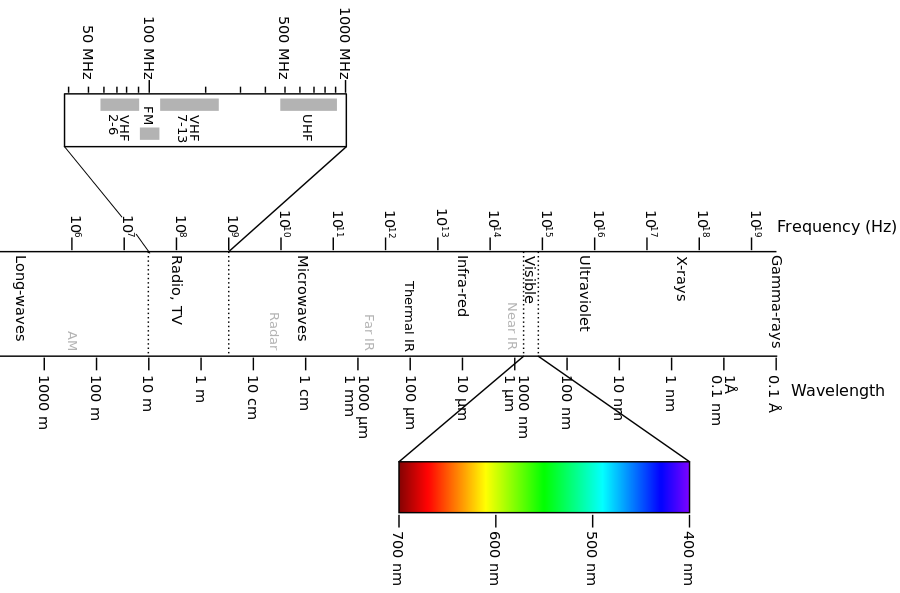
\includegraphics[width=\textwidth]{spectrum}
%  \caption{Το φάσμα της Ηλεκτρομαγνητικής Ακτινοβολίας}
%  \label{fig:spectrum}
%\end{figure}



\lettrine[findent=2pt]{\fbox{\textbf{Τ}}}{ο} λογισμικό που χρησιμοποιήθηκε για την υλοποίηση αυτής της εργασίας είναι το LabVIEW από την εταιρία National Instruments (ΝΙ). Συνεπώς, κρίνεται χρήσιμη μια σύντομη αναφορά σε αυτό και στον τρόπο που λειτουργεί. Καθώς το LabVIEW είναι ένα πολύ διαδεδομένο λογισμικό, με ευρεία χρήση στους κλάδους των μηχανικών, κάποιος που θέλει περισσότερες πληροφορίες μπορεί να τις βρει εύκολα στο διαδίκτυο. 
%Κάποιες πηγές που χρησιμοποιήθηκαν για τη συγγραφή αυτής της εργασίας είναι \cite{labview1}, \cite{labview2} και \cite{labview3}. 
Το LabVIEW (\emph{Laboratory Virtual Instrument Engineering Workbench}) είναι ένα περιβάλλον ανάπτυξης για μία οπτική γλώσσα προγραμματισμού. Σε αντίθεση με τα κοινά προγραμματιστικά περιβάλλοντα, στο LabVIEW δε χρησιμοποιείται κώδικας για να γραφτούν οι εντολές που θα εκτελεστούν αλλά γραφικά όπως κουτιά και σύμβολα. Για παράδειγμα, υπάρχουν πολλές οπτικές γλώσσες, που είναι γνωστές σαν γλώσσες ροής δεδομένων (\emph{dataflow}), που βασίζονται στην ιδέα "τετράγωνα και βέλη" (\emph{"boxes and arrows"}), όπου τα τετράγωνα (ή άλλου τύπου αντικείμενα) της οθόνης θεωρούνται οντότητες που συνδέονται από βέλη, γραμμές ή ακμές, που αναπαριστούν σχέσεις μεταξύ τους.

\subsection{Dataflow Programming}

Η οπτική γλώσσα προγραμματισμού του LabVIEW ονομάζεται ``G" και βασίζεται στη λογική του προγραμματισμού ροής δεδομένων που αναφέρθηκε προηγουμένως. Αυτό σημαίνει ότι αν υπάρχουν αρκετά δεδομένα διαθέσιμα σε μία συνάρτηση ή ένα σύνολο συναρτήσεων (\emph{subVI}), τότε αυτή η συνάρτηση ή το subVI θα εκτελεστεί. Η ροή της εκτέλεσης του προγράμματος καθορίζεται από τη δομή ενός σχηματικού διαγράμματος (\emph{block diagram}), που στην ουσία αποτελεί τον πηγαίο κώδικα του LabVIEW. Σε αυτό ο προγραμματιστής συνδέει διαφορετικές λειτουργίες (\emph{functions}) τραβώντας καλώδια. Αυτά τα καλώδια διαδίδουν τις μεταβλητές και κάθε λειτουργία μπορεί να εκτελεστεί μόλις όλα τα δεδομένα στην είσοδό της είναι διαθέσιμα. Δεδομένου ότι αυτό μπορεί να συμβαίνει για πολλαπλές λειτουργίες ταυτόχρονα, το LabVIEW μπορεί να εκτελεστεί εγγενώς παράλληλα.

\subsection{Graphical Programming}

Το LabVIEW ενσωματώνει τη δημιουργία διεπαφών χρήστη, που ονομάζονται εποπτικά πάνελ (\emph{front panels}). Ένα πρόγραμμα που έχει γραφτεί σε γλώσσα LabVIEW ονομάζεται εικονικό όργανο (\emph{VI}). Κάθε VI διαθέτει τρία στοιχεία: ένα block diagram, ένα front panel και ένα πάνελ σύνδεσης (\emph{connection panel}). Το τελευταίο χρησιμοποιείται για να αντιπροσωπεύει το VI στα block diagrams άλλων, καλώντας το VI. Το front panel κατασκευάζεται με χειριστήρια (\emph{controls}) και δείκτες (\emph{indicators}). Τα controls είναι είσοδοι: επιτρέπουν σε ένα χρήστη να παρέχει πληροφορίες στο VI. Τα indicators είναι έξοδοι: υποδηλώνουν ή εμφανίζουν τα αποτελέσματα με βάση τις εισόδους που δίδονται στο VI. Το block diagram, περιέχει τον γραφικό πηγαίο κώδικα. Όλα τα αντικείμενα που τοποθετούνται στο front panel εμφανίζονται στο block diagram ως τερματικά (\emph{terminals}). Το block diagram περιέχει επίσης δομές και λειτουργίες οι οποίες εκτελούν εργασίες στα controls και παρέχουν δεδομένα στα indicators. Οι δομές και οι λειτουργίες βρίσκονται στην παλέτα λειτουργιών και μπορούν να τοποθετηθούν στο block diagram. Οι συλλογικοί έλεγχοι, οι δείκτες, οι δομές και οι λειτουργίες θα αναφέρονται ως κόμβοι. Οι κόμβοι συνδέονται μεταξύ τους με τη χρήση καλωδίων, π.χ. δύο controls και μια ενδεικτική λυχνία μπορούν να συνδεθούν με τη χρήση της λειτουργίας προσθήκης (\emph{addition function}) έτσι ώστε η ένδειξη να εμφανίζει το άθροισμα των δύο controls. Έτσι, ένα VI μπορεί να λειτουργήσει είτε ως πρόγραμμα, με το front panel να λειτουργεί ως διεπαφή χρήστη, είτε, να χρησιμοποιηθεί ως κόμβος στο block diagram. Αυτό σημαίνει ότι κάθε VI μπορεί εύκολα να δοκιμαστεί πριν να ενσωματωθεί ως υπορουτίνα σε ένα μεγαλύτερο πρόγραμμα.

Η γραφική προσέγγιση επιτρέπει επίσης στους μη προγραμματιστές να χτίσουν προγράμματα με μεταφορά και απόθεση εικονικών αναπαραστάσεων του εργαστηριακού εξοπλισμού με τον οποίο είναι ήδη εξοικειωμένοι. Το περιβάλλον προγραμματισμού LabVIEW, με τα παραδείγματα και την τεκμηρίωση που περιλαμβάνονται, καθιστά απλή τη δημιουργία μικρών εφαρμογών. Αυτό είναι ένα πλεονέκτημα από τη μια πλευρά, αλλά υπάρχει επίσης ο κίνδυνος να υποτιμηθεί η εμπειρογνωμοσύνη που απαιτείται για τον προγραμματισμό ``G" υψηλής ποιότητας. Για σύνθετους αλγορίθμους ή κώδικα μεγάλης κλίμακας, είναι σημαντικό ο προγραμματιστής να έχει εκτεταμένη γνώση της σύνταξης του LabVIEW και της τοπολογίας της διαχείρισης μνήμης της. Τα πιο εξελιγμένα συστήματα ανάπτυξης LabVIEW προσφέρουν τη δυνατότητα δημιουργίας αυτόνομων εφαρμογών. Επιπλέον, είναι δυνατή η δημιουργία κατανεμημένων εφαρμογών, οι οποίες επικοινωνούν με ένα μοντέλο πελάτη -- εξυπηρετητή και έτσι είναι ευκολότερο να εφαρμοστούν λόγω της εγγενώς παράλληλης φύσης της προγραμματιστικής γλώσσας ``G". Ένα τυπικό περιβάλλον προγραμματισμού στο LabVIEW φαίνεται στο σχήμα \ref{fig:labview_example}

\begin{figure}[h!]
  \centering
  \begin{subfigure}[b]{0.4\linewidth}
    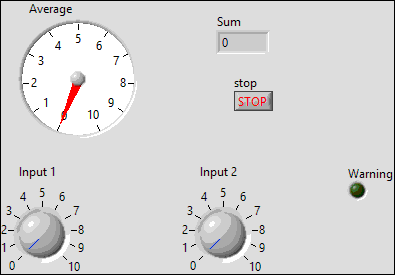
\includegraphics[width=\linewidth,height=5cm,keepaspectratio]{labview_fp}
    \caption{Front Panel}
  \end{subfigure}
  \begin{subfigure}[b]{0.4\linewidth}
    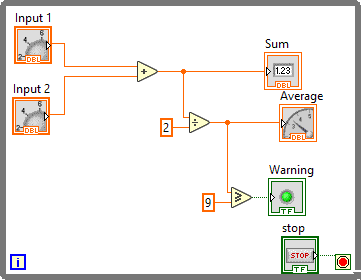
\includegraphics[width=\linewidth,height=5cm,keepaspectratio]{labview_bd}
    \caption{Block Diagram}
  \end{subfigure}
  \caption{Παράθυρα front panel και block diagram}
  \label{fig:labview_example}
\end{figure}

%\begin{figure}[h]
%  \centering
%  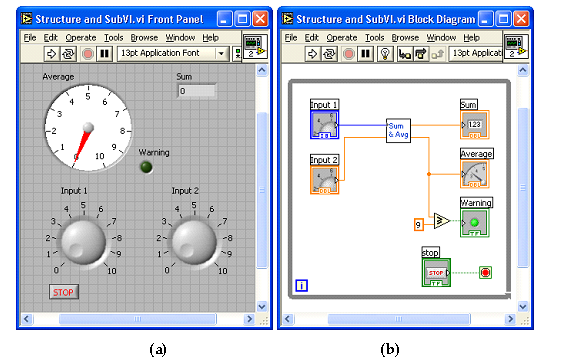
\includegraphics[width=\textwidth,height=5cm,keepaspectratio]{labview_example}
%  \caption{LabVIEW: Front Panel και Block Diagram}
%  \label{fig:labview_example}
%\end{figure}

%\lettrine[findent=2pt]{\fbox{\textbf{Ό}}}{πως} γνωρίζουμε από την επιστήμη της Φυσικής, όταν ένα σώμα ζεσταθεί αρκετά (π.χ. > 100 \degree C) αρχίζει και εκπέμπει ακτινοβολία και στο οπτικό φάσμα (πέραν του υπέρυθρου), ενώ αποκτά ταυτόχρονα μια ερυθρή όψη. Κατά το φαινόμενο αυτό, η ακτινοβολια που εκπέμπεται ανήκει τόσο στο υπέρυθρο, όσο και στο ορατό φάσμα της ηλεκτρομαγνητικής ακτινοβολίας και μάλιστα το χρώμα που αποκτά το σώμα συνδέεται άμεσα με τη θερμοκρασία στην οποία βρίσκεται. Οι περιοχές της υπέρυθρης και ορατής ακτινοβολίας, καταλαμβάνουν τις ζώνες $1mm - 700nm$ και $700nm - 390nm$ αντίστοιχα, όπως φαίνεται και στο σχήμα \ref{fig:spectrum}.


\clearemptydoublepage

\chapter{PID ελεγκτές}\label{ch:chap2}
%!TEX root = ../main.tex



\section{Εισαγωγή στους PID ελεγκτές}

\lettrine[findent=2pt]{\fbox{\textbf{Έ}}}{νας} αναλογικός-ολοκληρωτικός-παραγωγικός ελεγκτής (\emph{proportional-integral-derivative controller}) ή όπως είναι πιο γνωστός \emph{PID controller}, είναι ένας μηχανισμός ανάδρασης (\emph{feedback}) βρόχου ελέγχου (\emph{control loop}) που χρησιμοποιείται ευρέως σε βιομηχανικά συστήματα ελέγχου καθώς και σε μια ποικιλία άλλων εφαρμογών που απαιτούν συνεχή διαμορφωμένο έλεγχο. Η διαδικασία λειτουργίας είναι κοινή για όλους τους ελεγκτές αυτού του είδους. Ένας PID ελεγκτής υπολογίζει συνεχώς μια τιμή σφάλματος $e(t)$ ως διαφορά μεταξύ μιας επιθυμητής τιμής ρύθμισης (\emph{setpoint} ή \emph{SP}) και μεταξύ μιας μεταβλητής της διαδικασίας ύπο έλεγχο (\emph{process value} ή \emph{PV}) και εφαρμόζει μια διόρθωση βασισμένη στον αναλογικό, ολοκληρωτικό και παραγωγικό όρο του (\emph{P}, \emph{I}, \emph{D} αντίστοιχα) οι οποίοι δίνουν και στον ελεγκτή το όνομά του.\\
\linebreak
Στην πράξη, εφαρμόζει αυτόματα διορθωμένη και ακριβή διόρθωση σε μια λειτουργία ελέγχου. Ένα καθημερινό παράδειγμα είναι ο έλεγχος ταχύτητας σε οδικό όχημα. όπου εξωτερικές επιδράσεις, όπως κλίσεις, θα προκαλούσαν αλλαγές στην ταχύτητα του οχήματος. Ο αλγόριθμος PID επαναφέρει την ταχύτητα του αυτοκινήτου στην επιθυμητή από τον οδηγό τιμή της με τον βέλτιστο τρόπο, χωρίς καθυστέρηση ή υπέρβαση, ελέγχοντας την ισχύ εξόδου του κινητήρα του οχήματος.

\subsection{Ιστορική αναδρομή}

\subsubsection{Προέλευση}
Ο συνεχής έλεγχος, προτού καταστούν πλήρως κατανοητοί και εφαρμοσμένοι οι ελεγκτές PID, έχει μία από τις πηγές του στον φυγοκεντρικό ρυθμιστή ο οποίος χρησιμοποιεί περιστρεφόμενα βάρη για να ελέγξει μια διαδικασία. Αυτό είχε εφευρεθεί από τον Christian Huygens τον 17ο αιώνα για να ρυθμίσει το χάσμα μεταξύ των μυλόπετρων στους ανεμόμυλους ανάλογα με την ταχύτητα περιστροφής και έτσι να αντισταθμίσει την μεταβλητή ταχύτητα της τροφοδότησης των σιτηρών \cite{origin1}, \cite{origin2}.

Με την εφεύρεση της σταθερής ατμομηχανής υψηλής πίεσης, υπήρχε ανάγκη για αυτόματο έλεγχο ταχύτητας και ο αυτοδιαμορφωμένος ρυθμιστής ``κωνικού εκκρεμούς" του James Watt, ένα σύνολο περιστρεφόμενων χαλύβδινων σφαιρών προσαρτημένων σε κάθετο άξονα με βραχίονες σύνδεσης, έγινε πρότυπο της βιομηχανίας \cite{origin3}.

Ωστόσο, ο περιστρεφόμενος έλεγχος ταχύτητας του ρυθμιστή εξακολουθούσε να είναι μεταβλητός υπό συνθήκες μεταβαλλόμενου φορτίου, και έτσι το μειονέκτημα του ελέγχου που πλέον είναι γνωστός ως αναλογικός έγινε προφανές. Το σφάλμα μεταξύ της επιθυμητής ταχύτητας και της πραγματικής ταχύτητας αυξανόταν με την αύξηση του φορτίου. Τον $19^o$ αιώνα, η θεωρητική βάση για τη λειτουργία των ρυθμιστών περιγράφηκε για πρώτη φορά από τον James Clerk Maxwell το $1868$. Εξερεύνησε τη μαθηματική βάση για τη σταθερότητα του ελέγχου και προχώρησε σε έναν καλό δρόμο προς μια λύση, αλλά έκανε μια έκκληση σε μαθηματικούς να εξετάσουν το πρόβλημα \cite{origin3}, \cite{origin4}. Το πρόβλημα εξετάστηκε περαιτέρω από τον Edward Routh το $1874$, τον Charles Sturm και το $1895$ από τον Adolf Hurwitz, που όλοι συνέβαλαν στην καθιέρωση κριτηρίων σταθερότητας ελέγχου \cite{origin3}. Στην πράξη, οι ρυθμιστές ταχύτητας βελτιώθηκαν περαιτέρω, κυρίως από τον αμερικανικό επιστήμονα Willard Gibbs, ο οποίος το $1872$ ανέλυσε θεωρητικά τον κωνικό κυβερνήτη εκκρεμούς του Watt.

Περίπου εκείνη την εποχή, η εφεύρεση της τορπίλης Whitehead έθεσε ένα πρόβλημα ελέγχου το οποίο απαιτούσε ακριβή έλεγχο του βάθους λειτουργίας. Η χρήση μόνο ενός αισθητήρα πίεσης βάθους αποδείχθηκε ανεπαρκής και έτσι ένα εκκρεμές που μετρούσε το εμπρόσθιο και οπίσθιο βήμα της τορπίλης συνδυάστηκε με τη μέτρηση βάθους για να γίνει ο έλεγχος εκκρεμούς και υδροστάτη (\emph{pendulum-and-hydrostat control}). Ο έλεγχος πίεσης παρείχε μόνο ένα αναλογικό έλεγχο, το οποίο αν το κέρδος ελέγχου ήταν πολύ υψηλό, θα ήταν ασταθές και θα έπεφτε σε υπέρβαση, με σημαντική αστάθεια στη διατήρηση βάθους. Το εκκρεμές προσέθεσε αυτό που είναι τώρα γνωστό ως παράγωγο έλεγχο (\emph{derivative control}), το οποίο εξασθένισε τις ταλαντώσεις ανιχνεύοντας τη γωνία κατάδυσης / ανόδου της τορπίλης και επομένως τον ρυθμό μεταβολής του βάθους \cite{origin5}. Αυτή η εξέλιξη (που ονομάστηκε από το Whitehead ως ``\emph{Το Μυστικό}" για να μην δώσει καμιά ένδειξη για τη δράση της) ήταν περίπου το $1868$ \cite{origin6}.

Ένα άλλο πρώιμο παράδειγμα ελεγκτή τύπου PID αναπτύχθηκε από τον Elmer Sperry το $1911$ για την πλοήγηση, αν και το έργο του ήταν διαισθητικό και όχι μαθηματικό \cite{origin7}.

Η πρώτη θεωρητική ανάλυση και πρακτική εφαρμογή αφορούσε το αυτόματο σύστημα διεύθυνσης πλοίων, το οποίο αναπτύχθηκε από τις αρχές της δεκαετίας του $1920$ και μετά από τον μηχανικό Nicolas Minorsky \cite{origin8}. Ο Minorsky ερευνούσε και σχεδίαζε την αυτόματη καθοδήγηση πλοίων για το Πολεμικό Ναυτικό των ΗΠΑ και βάσισε την ανάλυσή του στις παρατηρήσεις ενός πηδαλιούχου. Σημείωσε ότι ο πηδαλιούχος κατεύθυνε το πλοίο με βάση όχι μόνο το τρέχον σφάλμα πορείας, αλλά και το λάθος του παρελθόντος, καθώς και τον τρέχοντα ρυθμό αλλαγής \cite{origin9}. Αυτό μοντελοποιήθηκε μαθηματικά από τον Minorsky \cite{origin3}. Ο στόχος του ήταν η σταθερότητα, όχι ο γενικός έλεγχος, ο οποίος απλοποίησε σημαντικά το πρόβλημα. Ενώ ο αναλογικός έλεγχος παρείχε σταθερότητα έναντι μικρών διαταραχών, ήταν ανεπαρκής για να αντιμετωπίσει μια σταθερή διαταραχή (λόγω σφάλματος σταθερής κατάστασης), η οποία απαιτούσε την προσθήκη του ολοκληρωτικού όρου. Τέλος, ο παράγωγος όρος προστέθηκε για να βελτιώσει τη σταθερότητα και τον έλεγχο.

Διεξήχθησαν δοκιμές στο USS New Mexico, με τον ελεγκτή να ελέγχει τη γωνιακή ταχύτητα (όχι τη γωνία) του πηδαλίου. Ο έλεγχος PI απέδωσε σταθερή στροφή (γωνιακό σφάλμα) $±2\degree$. Η προσθήκη του στοιχείου D οδήγησε σε σφάλμα εκτροπής $±{1/6}\degree$, καλύτερα από ότι θα μπορούσαν να επιτύχουν οι περισσότεροι πηδαλιούχοι \cite{origin10}.

Το Πολεμικό Ναυτικό τελικά δεν υιοθέτησε το σύστημα, λόγω της αντίστασης του προσωπικού. Παρόμοια εργασία πραγματοποιήθηκε και δημοσιεύθηκε από αρκετούς άλλους στη δεκαετία του $1930$.

\subsubsection{Βιομηχανικός έλεγχος}
Η ευρεία χρήση των ελεγκτών ανάδρασης δεν κατέστη εφικτή μέχρις ότου αναπτύχθηκαν ενισχυτές υψηλού κέρδους και μεγάλης ζώνης (\emph{wideband high-gain amplifiers}) για να χρησιμοποιηθεί η έννοια της αρνητικής ανάδρασης. Αυτοί είχαν αναπτυχθεί στην ηλεκτρονική τηλεφωνική μηχανική από τον Harold Black στα τέλη της δεκαετίας του $1920$, αλλά δεν δημοσιεύθηκε μέχρι το $1934$ \cite{origin3}. Ανεξάρτητα, ο Clesson E Mason της εταιρείας Foxboro, το $1930$, εφηύρε έναν ευρείας ζώνης πνευματικό ελεγκτή, συνδυάζοντας τον πνευματικό ενισχυτή με ακροφύσιο και πτερύγιο υψηλού κέρδους, που είχε εφευρεθεί το $1914$, με αρνητική ανάδραση από την έξοδο του ελεγκτή. Αυτό αύξησε δραματικά το γραμμικό εύρος λειτουργίας του ακροφυσίου και του ενισχυτή πτερυγίου και ο ολοκληρωμένος έλεγχος μπορούσε επίσης να προστεθεί με τη χρήση μιας βαλβίδας εξαέρωσης ακριβείας και ενός φυσητήρα. Το αποτέλεσμα ήταν ο ελεγκτής "Stabilog" ο οποίος έδωσε αναλογικές και ολοκληρωμένες λειτουργίες χρησιμοποιώντας ανατροφοδοτούμενους φυσητήρες \cite{origin3}. Αργότερα ο παράγωγος όρος προστέθηκε από ένα άλλο φυσητήρα και ρυθμιζόμενο στόμιο.

Από το $1932$ και μετά, η χρήση ευρυζωνικών ελεγκτών αυξήθηκε ραγδαία σε ποικίλες εφαρμογές ελέγχου. Ο πεπιεσμένος αέρας χρησιμοποιήθηκε τόσο για την παραγωγή της εξόδου του ελεγκτή όσο και για την τροφοδοσία της συσκευής διαμόρφωσης της διαδικασίας, όπως μια βαλβίδα ελέγχου που λειτουργεί με διαφράγματα. Ήταν απλές συσκευές χαμηλής συντήρησης που λειτουργούσαν καλά σε σκληρό βιομηχανικό περιβάλλον και δεν παρουσίαζαν κίνδυνο έκρηξης σε επικίνδυνες τοποθεσίες. Ήταν το βιομηχανικό πρότυπο για πολλές δεκαετίες μέχρι την εμφάνιση διακριτών ηλεκτρονικών ελεγκτών και κατανεμημένων συστημάτων ελέγχου.

\begin{figure}[h]
  \centering
  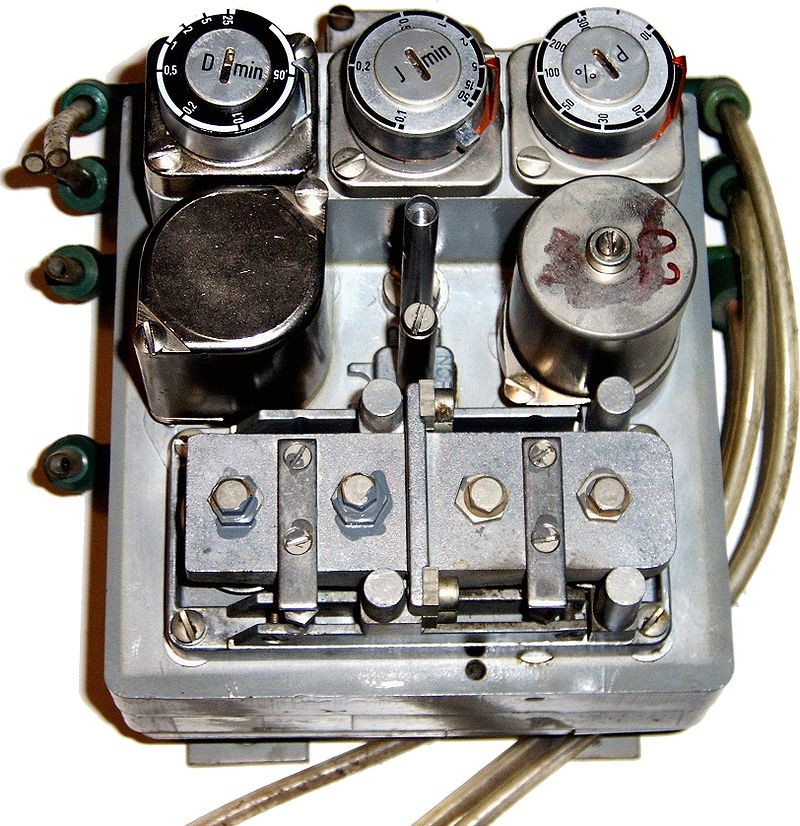
\includegraphics[width=\textwidth]{pneumatic_pid}
  \caption{Πνευματικός ελεγκτής PID. Οι συντελεστές των "τριών όρων" Ρ, Ι και D ρυθμίζονται από τους διακόπτες στην κορυφή}
  \label{fig:pneumatic_pid}
\end{figure}

Στη δεκαετία του $1950$, όταν οι ηλεκτρονικοί ενισχυτές υψηλού κέρδους έγιναν φτηνοί και αξιόπιστοι, οι ηλεκτρονικοί ελεγκτές PID έγιναν δημοφιλείς και χρησιμοποιήθηκαν σήματα ρεύματος βρόχου $4-20 mA$ τα οποία εξομοιώνουν το πνευματικό πρότυπο. Ωστόσο, οι ενεργοποιητές πεδίου (\emph{field actuators}) εξακολουθούν να χρησιμοποιούν ευρέως το πνευματικό πρότυπο λόγω των πλεονεκτημάτων της πνευματικής κινητήριας δύναμης για τις βαλβίδες ελέγχου στα περιβάλλοντα των μονάδων επεξεργασίας.

\subsubsection{Ηλεκτρονικοί αναλογικοί ελεγκτές}
Οι ηλεκτρονικοί αναλογικοί βρόχοι ελέγχου PID βρίσκονταν συχνά μέσα σε πιο σύνθετα ηλεκτρονικά συστήματα, όπως για παράδειγμα η τοποθέτηση της κεφαλής μιας μονάδας σκληρού δίσκου, η ρύθμιση της ισχύος ενός τροφοδοτικού ή ακόμα και το κύκλωμα ανίχνευσης κίνησης ενός σύγχρονου σεισμομέτρου. Οι διακριτοί ηλεκτρονικοί αναλογικοί ελεγκτές έχουν αντικατασταθεί σε μεγάλο βαθμό από ψηφιακούς ελεγκτές που χρησιμοποιούν μικροελεγκτές ή FPGA, για την εφαρμογή αλγορίθμων PID. Ωστόσο, διακριτοί αναλογικοί ελεγκτές PID εξακολουθούν να χρησιμοποιούνται σε εξειδικευμένες εφαρμογές που απαιτούν απόδοση υψηλού εύρους ζώνης και χαμηλού θορύβου, όπως ελεγκτές με λέιζερ-δίοδο \cite{origin11}.

%Στη συνέχεια χρησιμοποιήθηκε για τον αυτόματο έλεγχο της διαδικασίας στη μεταποιητική βιομηχανία, όπου εφαρμόστηκε ευρέως σε πνευματικούς, και στη συνέχεια ηλεκτρονικούς, ελεγκτές. Σήμερα υπάρχει γενική χρήση της ιδέας PID σε εφαρμογές που απαιτούν ακριβή και βελτιστοποιημένο αυτόματο έλεγχο.

\subsection{Χρησιμότητα PID ελεγκτών}

Ο PID ελεγκτής έχει διάφορα σημαντικά χαρακτηριστικά: παρέχει ανατροφοδότηση ελέγχου, έχει την ικανότητα να εξαλείφει το σφάλμα μόνιμης κατάστασης (\emph{steady-state error}) μέσω του ολοκληρωτικού του όρου, μπορεί να προβλέπει το μελλοντικό σφάλμα μέσω του παραγωγικού του όρου. Οι PID ελεγκτές παρέχουν ικανοποιητικό έλεγχο σε πολλά προβλήματα ελέγχου, ειδικά όταν οι δυναμικές που διέπουν τη διεργασία είναι ήπιες και οι απαιτήσεις ελέγχου μέτριες. Οι ελεγκτές αυτού του είδους έρχονται σε αρκετές διαφορετικές μορφές. Υπάρχουν αυτόνομα συστήματα μέσα σε κουτιά για έναν ή περισσότερους βρόχους και παράγονται εκατοντάδες χιλιάδες μονάδες κάθε χρόνο. Ο PID έλεγχος είναι σημαντικό στοιχείο ενός κατανεμημένου συστήματος ελέγχου. Οι ελεγκτές είναι επίσης ενσωματωμένοι σε πολλά, ειδικού σκοπού, συστήματα ελέγχου. Στον έλεγχο διεργασιών (\emph{process control}), περισσότερο από το $95\%$ των βρόχων ελέγχου είναι PID τύπου (οι περισσότεροι βρόχοι είναι στην πραγματικότητα PI ελέγχου).

Η δημοτικότητα του PID οφείλεται σε μεγάλο βαθμό στην ευκολία εφαρμογής και την αποτελεσματικότητά του. Το κίνητρο για τη χρήση του PID προέρχεται από την αποδοτικότητα του κόστους υλοποίησής του: ο ελεγκτής PID σπάνια αποτελεί ένα βέλτιστο ελεγκτή αλλά είναι αρκετά καλός στις περισσότερες περιπτώσεις και έτσι το πρόσθετο κόστος και η πολυπλοκότητα ενός βέλτιστου ελεγκτή δεν αξίζουν την οριακή αύξηση στην απόδοση. Επιπλέον, ο έλεγχος PID δεν απαιτεί βαθιά κατανόηση των υποκείμενων λειτουργιών μιας διαδικασίας. Το μόνο που έχει σημασία είναι ότι μερικές μετρούμενες μεταβλητές της διαδικασίας να μπορούν να επηρεαστούν έντονα από ορισμένες ελεγχόμενες μεταβλητές. Επίσης ένας PID ελεγκτής μπορεί εύκολα να μεταφερθεί από διεργασία σε διεργασία. Το μόνο που χρειάζεται είναι να προσαρμοστούν τα κέρδη των όρων του και τα όρια της εξόδου του έτσι ώστε να ταιριάζουν στην καινούρια διεργασία. Ο PID έλεγχος χρησιμοποιείται στο χαμηλότερο επίπεδο: ο πολλαπλών μεταβλητών ελεγκτής (\emph{multivariable controller}) δίνει το σημείο λειτουργίας στους ελεγκτές στο χαμηλότερο επίπεδο. Ο PID ελεγκτής μπορεί λοιπόν να ειπωθεί ότι αποτελεί το ``ψωμί και βούτυρο" της μηχανικής ελέγχου. Είναι, συνεπώς, ένα σημαντικό στοιχείο στην εργαλειοθήκη κάθε μηχανικού ελέγχου. 

Οι PID ελεγκτές έχουν επιβιώσει πολλές αλλαγές στην τεχνολογία πηγαίνοντας από τη χρήση πνευματικών συστημάτων στη χρήση μικροεπεξεργαστών μέσω ηλεκτρονικών σωλήνων, τρανζίστορ, ολοκληρωμένων κυκλωμάτων. Οι μικροεπεξεργαστές είχαν μεγάλη επίδραση στους PID ελεγκτές. Βασικά όλοι οι PID ελεγκτές σήμερα κατασκευάζονται με τη χρήση μικροεπεξεργαστών. Αυτό έδωσε τη δυνατότητα να συμπεριληφθούν επιπλέον χαρακτηριστικά στους PID ελεγκτές, όπως η αυτο-ρύθμισή τους που υλοποιείται σε αυτή την εργασία.

\section{Αρχές λειτουργίας}

\lettrine[findent=2pt]{\fbox{\textbf{Ο}}}{} PID ελεγκτής είναι, κατά πολύ, ο πιο κοινός αλγόριθμος ελέγχου. Οι περισσότεροι βρόχοι ανάδρασης ελέγχονται από αυτόν τον αλγόριθμο ή από διαφοροποιήσεις του. Συνεπώς ο έλεγχος αυτός έχει διάφορους τρόπους με τους οποίους μπορεί να αντιμετωπιστεί. Μπορεί να θεωρείται ως συσκευή η οποία λειτουργεί με κάποιους εμπειρικούς κανόνες ή μπορεί και να προσεγγιστεί αναλυτικά. Σε αυτή την ενότητα θα παρουσιαστούν ο βασικός αλγόριθμος καθώς και οι μηχανισμοί που διέπουν τη λειτουργία του PID ελεγκτή. Καθώς αυτή η ενότητα αποτελεί μια σύντομη εισαγωγή στη θεωρία του PID ελεγκτή, η ανάλυση που θα γίνει είναι σύντομη και απαιτεί το ελάχιστο μαθηματικό υπόβαθρο. Όποιος ενδιαφέρεται για μια εις βάθος μαθηματική ανάλυση μπορεί να ανατρέξει στην πηγή \cite{astrom}.

\subsection{H Ανάδραση}

Όπως οι περισσότεροι ελεγκτές, έτσι και ο PID, βασίζεται στην έννοια της ανατροφοδότησης ή ανάδρασης. Συνεπώς αξίζει να γίνει μια σύντομη αναφορά στο τι είναι ανάδραση και πώς λειτουργεί. Η ανάδραση είχε μεγάλη επιρροή στην εξέλιξη της τεχνολογίας σε διάφορα πεδία, μεταξύ αυτών και ο αυτόματος έλεγχος. Χάριν απλότητας, ας υποθέσουμε ότι σε μία διαδικασία, αν αυξηθεί η έξοδος του ελεγκτή (\emph{manipulated variable}) τότε θα αυξηθεί και η τιμή της μεταβλητής της διαδικασίας που μας ενδιαφέρει (\emph{process variable}). Με αυτό το σκεπτικό, η ανάδραση μπορεί να περιγραφεί ως:
\begin{quote}
Αύξησε τη manipulated variable όταν η process variable είναι χαμηλότερη από την επιθυμητή τιμή και μείωσε τη manipulated variable όταν η process variable είναι μεγαλύτερη από την επιθυμητή τιμή.
\end{quote}
Αυτού του είδους η ανάδραση ονομάζεται αρνητική (\emph{negative feedback}) γιατί η manipulated variable κινείται αντίθετα από την process variable. Το Σχήμα \ref{fig:feedback} δείχνει ένα τυπικό παράδειγμα αρνητικής ανάδρασης. Ο λόγος που η αρνητική ανάδραση είναι τόσο σημαντική είναι επειδή κάνει την process variable να πλησιάζει την επιθυμητή τιμή, παρά την ύπαρξη διαταραχών και διακυμάνσεων στα χαρακτηριστικά της διεργασίας.

\begin{figure}[h]
  \centering
  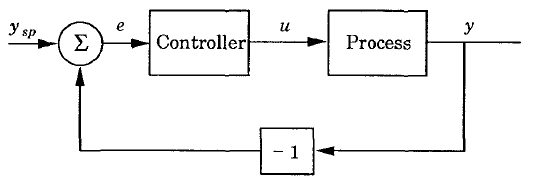
\includegraphics[width=\textwidth]{feedback}
  \caption{Δομικό διάγραμμα μιας διεργασίας με αρνητική ανάδραση}
  \label{fig:feedback}
\end{figure}

\subsection{Αναλογικός Όρος}

Ο αναλογικός όρος παράγει ένα σήμα εξόδου το οποίο είναι ανάλογο στην τρέχουσα τιμή του σφάλματος. Αυτό επιτυγχάνεται πολλαπλασιάζοντας το σφάλμα $e(t)=y_{sp}-y$ με ένα συντελεστή $K_p$ που ονομάζεται αναλογική σταθερά κέρδους (\emph{proportional gain constant}). Ο αναλογικός όρος συνεπώς δίνεται από τη σχέση:
\begin{equation}
P_{out}=K_p e(t)
\label{eq:p_out}
\end{equation}
Ένα υψηλό αναλογικό κέρδος έχει ως αποτέλεσμα μια μεγάλη αλλαγή στην έξοδο για μια δεδομένη αλλαγή στο σφάλμα. Εάν το αναλογικό κέρδος είναι πολύ υψηλό, το σύστημα μπορεί να γίνει ασταθές (βλ. Το τμήμα σχετικά με τη ρύθμιση βρόγχου). Σε αντίθεση, ένα μικρό κέρδος έχει ως αποτέλεσμα μια μικρή απόκριση εξόδου σε ένα μεγάλο σφάλμα εισόδου και έναν λιγότερο ανταποκρίσιμο ή λιγότερο ευαίσθητο ελεγκτή. Αν το αναλογικό κέρδος είναι πολύ χαμηλό, η ενέργεια ελέγχου μπορεί να είναι πολύ μικρή όταν οφείλεται σε διαταραχές του συστήματος. Στις περισσότερες εφαρμογές ελέγχου, ο αναλογικός όρος είναι αυτός που συνεισφέρει το μεγαλύτερο μέρος στην έξοδο του ελεγκτή.

Επειδή ο αναλογικός όρος επιδρά στην τρέχουσα τιμή του σφάλματος, ένας αναλογικός ελεγκτής πάντα παρουσιάζει ένα σφάλμα μόνιμης κατάστασης (\emph{steady state error}). Εξαίρεση αποτελεί η περίπτωση που η επιθυμητή τιμή είναι η τιμή στην οποία ο αναλογικός όρος ισούται με το μηδέν. Στο Σχήμα \ref{fig:proportional} φαίνεται η επίδραση μόνο του αναλογικού όρου σε μια διεργασία. Για την εξάλειψη του σφάλματος μόνιμης κατάστασης χρησιμοποιούμε τον όρο που αναφέρεται στη συνέχεια.

\begin{figure}[h]
  \centering
  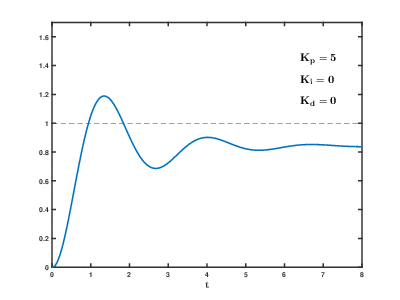
\includegraphics[width=\textwidth]{proportional}
  \caption{Επίδραση του αναλογικού όρου σε μια διεργασία}
  \label{fig:proportional}
\end{figure}

\subsection{Ολοκληρωτικός Όρος}

Η συμβολή του ολοκληρωτικού όρου είναι ανάλογη τόσο με το μέγεθος του σφάλματος όσο και με τη διάρκεια του. Το ολοκλήρωμα ενός ελεγκτή PID είναι το άθροισμα του στιγμιαίου σφάλματος με την πάροδο του χρόνου και δίνει τη συσσωρευμένη μετατόπιση που θα έπρεπε να είχε διορθωθεί προηγουμένως. Το συσσωρευμένο σφάλμα στη συνέχεια πολλαπλασιάζεται με το ολοκληρωτικό κέρδος ($K_i$) και προστίθεται στην έξοδο του ελεγκτή. Ο ολοκληρωτικός όρος δίνεται από τη σχέση:
\begin{equation}
I_{out}=K_i \int_{0}^{t} e(\tau)d\tau
\label{eq:i_out}
\end{equation}
όπου $\tau$ είναι η μεταβλητή ολοκλήρωσης και παίρνει τιμές από το $0$ έως την τρέχουσα χρονική στιγμή $t$. Έτσι, αν η εφαρμοζόμενη δράση δεν είναι αρκετή για να φέρει το σφάλμα στο μηδέν, αυτή η δράση θα αυξηθεί με το πέρασμα του χρόνου. Επίσης ο ολοκληρωτικός όρος επιταχύνει την κίνηση της process variable προς την επιθυμητή τιμή. Ένας καθαρός ολοκληρωτικός ελεγκτής ``I" θα μπορούσε να φέρει το σφάλμα στο μηδέν, ωστόσο θα είχε πολύ αργή αντίδραση στην αρχή (επειδή η δράση θα ήταν μικρή, και θα χρειαζόταν χρόνο για να γίνει σημαντική), βίαιη (η δράση αυξάνεται όσο το σφάλμα είναι θετικό, ακόμη και αν το σφάλμα έχει αρχίσει να πλησιάζει το μηδέν) και αργή να τελειώσει (όταν το σφάλμα αλλάζει πρόσημο, αυτό για κάποιο χρονικό διάστημα μόνο θα μειώνει τη δύναμη της δράσης του ελεγκτή και δε θα το κάνει να αλλάζει και αυτή πρόσημο), προκαλώντας υπέρβαση και ταλαντώσεις. Επιπλέον, θα μπορούσε να προκαλέσει το σύστημα να αποκριθεί ακόμα και αν υπάρχει ήδη μηδενικό σφάλμα καθώς θυμάται ότι το σύστημα είχε σφάλμα και έτσι θα μπορούσε να προκαλέσει μια ενέργεια όταν αυτή δεν είναι απαραίτητη. Το Σχήμα \ref{fig:integral} δείχνει πώς η προσθήκη ενός ολοκληρωτικού όρου εξαλείφει το σφάλμα μόνιμης κατάστασης που δεν κατάφερε να εξαλείψει ο αναλογικός όρος αλλά ταυτόχρονα εισάγει ταλαντώσεις στο σύστημα.

\begin{figure}[h]
  \centering
  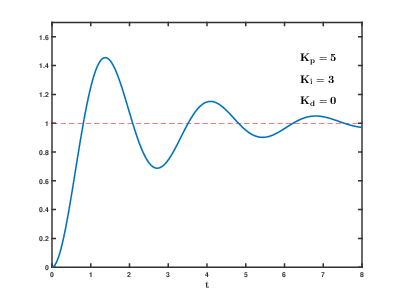
\includegraphics[width=\textwidth]{integral}
  \caption{Εφαρμογή του ολοκληρωτικού όρου στην προηγούμενη απόκριση κρατώντας το αναλογικό κέρδος σταθερό}
  \label{fig:integral}
\end{figure}

\subsection{Παράγωγος Όρος}

Η παράγωγος του σφάλματος της διαδικασίας υπολογίζεται καθορίζοντας την κλίση του σφάλματος με την πάροδο του χρόνου και πολλαπλασιάζοντας αυτόν τον ρυθμό μεταβολής με το κέρδος του παραγώγου $K_d$. Το μέγεθος της συμβολής του παραγώγου όρου στη συνολική δράση ελέγχου ονομάζεται παράγωγο κέρδος (\emph{derivative gain}), $K_d$. Ο παράγωγος όρος δίνεται από τη σχέση:
\begin{equation}
D_{out}=K_d \frac{de(t)}{dt}
\label{eq:dout}
\end{equation}
Ένας παράγωγος όρος δεν λαμβάνει υπόψιν του το σφάλμα (αυτό σημαίνει ότι δεν μπορεί να το φτάσει στο μηδέν: ένας καθαρός ελεγκτής ``D" δεν μπορεί να φέρει το σύστημα στην επιθυμητή τιμή του), αλλά το ρυθμό αλλαγής του σφάλματος, προσπαθώντας να φέρει αυτόν τον ρυθμό στο μηδέν. Στόχος του είναι η τροχιά του σφάλματος να γίνει μια οριζόντια γραμμή, αποσβένοντας την εφαρμοζόμενη δύναμη και μειώνοντας έτσι την υπέρβαση (\emph{overshoot}). Η εφαρμογή υπερβολικής ώθησης όταν το σφάλμα είναι μικρό και συνεχίζει να μειώνεται θα οδηγήσει σε υπέρβαση. Μετά την υπέρβαση, αν ο ελεγκτής εφαρμόσει μια μεγάλη διόρθωση στην αντίθετη κατεύθυνση και επανειλημμένα υπερβεί την επιθυμητή θέση, η έξοδος θα ταλαντώνεται γύρω από την επιθυμητή τιμή είτε σε ένα σταθερό, αναπτυσσόμενο ή σε αποσβεννούμενο ημιτονοειδές. Εάν το πλάτος των ταλαντώσεων αυξάνεται με το χρόνο, το σύστημα είναι ασταθές. Εάν μειώνεται, το σύστημα είναι σταθερό. Εάν οι ταλαντώσεις διατηρούν σταθερό πλάτος, το σύστημα είναι οριακά σταθερό. Ο παράγωγος όρος προβλέπει τη συμπεριφορά του συστήματος και επομένως βελτιώνει τον χρόνο που απαιτείται για να ηρεμήσει το σύστημα (\emph{settling time}) καθώς και τη σταθερότητα του συστήματος \cite{michigan}, \cite{wescott}. Ένα ιδανικός παράγωγος ελεγκτής δεν είναι αιτιατός, και έτσι οι εφαρμογές των PID ελεγκτών περιλαμβάνουν ένα πρόσθετο φίλτρο χαμηλής διέλευσης (\emph{low-pass filter}) για τον παράγωγο όρο για να περιορίσουν το κέρδος και το θόρυβο υψηλής συχνότητας. Ο παράγωγος όρος χρησιμοποιείται πολύ πιο σπάνια στην πράξη από τους άλλους δύο όρους (P και I), λόγω της μεταβλητής επίδρασής του στη σταθερότητα του συστήματος σε πραγματικές εφαρμογές. Το Σχήμα \ref{fig:derivative} δείχνει πώς βελτιώθηκε η συνολική απόκριση του συστήματος και εξαλείφθηκαν οι ταλαντώσεις που είχε εισάγει ο ολοκληρωτικός όρος με την προσθήκη του όρου παραγώγου.

\begin{figure}[h]
  \centering
  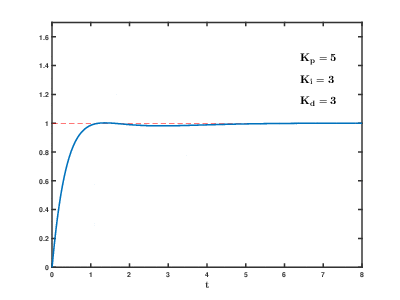
\includegraphics[width=\textwidth]{derivative}
  \caption{Εφαρμογή του όρου παραγώγου στην προηγούμενη απόκριση κρατώντας τα άλλα κέρδη σταθερά}
  \label{fig:derivative}
\end{figure}

\subsection{Εξίσωση του PID ελεγκτή}

Οι τρεις όροι που αναλύθηκαν παραπάνω είναι αυτοί που δίνουν στον ελεγκτή το όνομά του. Το άθροισμα των τριών αυτών όρων αποτελεί τη μεταβλητή που μεταχειρίζεται ο ελεγκτής (\emph{manipulated variable}) και ισούται με την έξοδό του. Ορίζοντας ως $u(t)$ την έξοδο του ελεγκτή και αθροίζοντας τις εξισώσεις \ref{eq:p_out}, \ref{eq:i_out} και \ref{eq:dout} η τελική μορφή του είναι:
\begin{equation}
u(t)=MV(t)=K_p e(t) + K_i \int_{0}^{t} e(\tau)d\tau + K_d \frac{de(t)}{dt}
\label{eq:parallel_pid}
\end{equation}
Αυτή η μορφή του PID είναι γνωστή ως παράλληλη (\emph{parallel}). Η μορφή του PID που χρησιμοποιείται περισσότερο στη βιομηχανία και η οποία χρησιμοποιήθηκε και σε αυτή την εργασία είναι η τυποποιημένη μορφή (\emph{standard form}). Σε αυτή τη μορφή το κέρδος του αναλογικού όρου $K_p$ εφαρμόζεται και στους άλλους δύο όρους και έτσι η εξίσωση που προκύπτει είναι η:
\begin{equation}
u(t)=MV(t)=K_p \left( e(t) + \frac{1}{T_i}\int_{0}^{t} e(\tau)d\tau + T_d\frac{de(t)}{dt} \right)
\label{eq:standard_pid}
\end{equation}
όπου $\boldsymbol{T_i}$ είναι ο χρόνος ολοκλήρωσης και $\boldsymbol{T_d}$ είναι ο χρόνος παραγώγισης. Σε αυτή τη μορφή, οι παράμετροι έχουν σαφή φυσική σημασία. Συγκεκριμένα, η εσωτερική άθροιση παράγει μια νέα μοναδική τιμή σφάλματος η οποία αντισταθμίζεται για μελλοντικά και παρελθόντα σφάλματα. Η προσθήκη των αναλογικών και παραγώγων συνιστωσών προβλέπει την τιμή σφάλματος σε $T_d$ δευτερόλεπτα (ή δείγματα) στο μέλλον, υποθέτοντας ότι ο έλεγχος βρόχου παραμένει αμετάβλητος. Το ολοκληρωτικό στοιχείο προσαρμόζει την τιμή σφάλματος για να αντισταθμίσει το άθροισμα όλων των παρελθόντων σφαλμάτων, με σκοπό την πλήρη εξάλειψή τους $T_i$ δευτερόλεπτα (ή δείγματα). Η προκύπτουσα αντισταθμισμένη τιμή μοναδικού σφάλματος κλιμακώνεται από το μοναδικό κέρδος $K_p$.

Οι συντελεστές της εξίσωσης (\ref{eq:parallel_pid}) με αυτούς της εξίσωσης (\ref{eq:standard_pid}) συνδέονται με τις σχέσεις: $\boldsymbol{K_i=\frac{K_p}{T_i}}$ και $\boldsymbol{K_d=K_p T_d}$. Η παράλληλη μορφή, όπου οι παράμετροι αντιμετωπίζονται ως απλά κέρδη, είναι η πιο γενική και ευέλικτη μορφή. Ωστόσο, είναι επίσης η μορφή όπου οι παράμετροι αυτοί έχουν τη λιγότερη φυσική ερμηνεία και γενικά προορίζονται για θεωρητική ανάλυση του PID ελεγκτή. Η τυποποιημένη μορφή, παρά το γεγονός ότι είναι λίγο πιο περίπλοκη μαθηματικά, είναι πιο συνηθισμένη στη βιομηχανία.

\paragraph{\fbox{Σύνοψη}}
Ο PID ελεγτκής έχει τρεις όρους. Ο αναλογικός όρος (\emph{``P"}) αφορά τον αναλογικό έλεγχο και επιδρά στο τρέχον σφάλμα. Ο ολοκληρωτικός όρος (\emph{``I"}) παρέχει μια δράση ελέγχου που είναι ανάλογη στο χρονικό ολοκλήρωμα του σφάλματος. Αυτό εξασφαλίζει ότι το σφάλμα μόνιμης κατάστασης γίνεται μηδενικό. Ο παράγωγος όρος (\emph{``D"}) είναι ανάλογος της χρονικής παραγώγου του σφάλματος. Αυτός ο όρος προβλέπει το μελλοντικό σφάλμα. Εκτός από αυτές τις δύο μορφές του PID υπάρχουν και άλλες, η καθεμία με διαφορετικές ιδιότητες αλλά οι δύο που αναφέρθηκαν είναι οι πιο γνωστές. Κάποιος που θέλει να μελετήσει και τις άλλες μπορεί να απευθυνθεί στην πηγή \cite{astrom}.

\subsection{Τροποποιήσεις του PID αλγορίθμου}

\subsubsection{Integral Windup}
Όταν σχεδιάζεται ένας πρακτικός PID ελεγκτής που θα ελέγχει πραγματικούς ενεργοποιητές όπως βαλβίδες, διακόπτες κτλ, θα πρέπει να λαμβάνονται υπόψιν και οι περιορισμοί του εξοπλισμού αυτού. Για παράδειγμα ένας κινητήρας έχει περιορισμένη ταχύτητα, μια βαλβίδα έχει όρια στο πόσο ανοιχτή ή πόσο κλειστή μπορεί να είναι και ούτω καθεξής. Συνεπώς, αν ένα σύστημα δεν μπορεί να φτάσει την επιθυμητή τιμή χωρίς να ξεπεράσει αυτά τα όρια τότε θα υπάρχει πάντα ένα σφάλμα μόνιμης κατάστασης, ακόμα και αν έχει προστεθεί ο ολοκληρωτικός όρος στον PID ελεγκτή. Αυτό έχει σαν αποτέλεσμα ο ολοκληρωτικός όρος να συνεχίζει να συσσωρεύει σφάλμα και έτσι αυτός μπορεί να γίνει πολύ μεγάλος και να οδηγήσει το σύστημα σε ανεπιθύμητη συμπεριφορά. Αυτό αναφέρεται στη διεθνή βιβλιογραφία ως \textbf{\emph{integral windup}}. Αυτό το πρόβλημα μπορεί να αντιμετωπιστεί με κάποια από τις ακόλουθες τροποποιήσεις στο βασικό αλγόριθμο:
\begin{itemize}
\item Απενεργοποίηση της ολοκλήρωσης έως ότου η μεταβλητή της διεργασίας εισέλθει στην ελεγχόμενη περιοχή
\item Αποτροπή της συσσώρευσης του ολοκληρωτικού όρου πάνω ή κάτω από τα προκαθορισμένα όρια
\item Υπολογισμός εκ των υστέρων του ολοκληρωτικού όρου για τον περιορισμό της εξόδου του ελεγκτή εντός εφικτών ορίων
\end{itemize}

\subsubsection{Bumpless λειτουργία}
Διάφορες αλλαγές μπορεί να επέλθουν σε έναν PID που είναι ενεργός. Μπορεί να αλλάξουν οι παράμετροί του ή να αλλάξει η λειτουργία του από χειροκίνητη σε αυτόματη. Οι ελεγκτές PID υλοποιούνται συχνά με ένα χαρακτηριστικό ``εξομάλυνσης" έτσι ώστε η έξοδός τους να μεταβάλλεται με ομαλό τρόπο κατά τη διάρκεια αυτών των αλλαγών \cite{douglas}.

\subsubsection{Περισσότερες τροποποιήσεις}
Φυσικά μετά από τόσα χρόνια εφαρμογής του PID αλγορίθμου στη βιομηχανία, πολλές εναλλακτικές μορφές του έχουν προταθεί, πέρα από αυτές τις δύο προαναφερθέντες. Η καθεμία από αυτές τις τροποποιήσεις βελτιώνει πολλά από τα προβλήματα του βασικού αλγορίθμου. Κάποιος που θέλει να ενημερωθεί για όλες τις τροποποιήσεις του αλγορίθμου αναλυτικά, καλείται να ανατρέξει στην πηγή \cite{astrom}.

%\section{Ρύθμιση του PID ελεγκτή}
%
%\lettrine[findent=2pt]{\fbox{\textbf{Η}}}{} ρύθμιση του PID ελεγκτή έχει να κάνει με την απόδοση τιμών στο συντελεστή κάθε όρου, έτσι ώστε καθένας από αυτούς να επηρεάσει θετικά την απόκριση του συστήματος, ενώ ταυτόχρονα να μετριαστούν όσο γίνεται περισσότερο τα αρνητικά του κάθε όρου. Ο τύπος της διεργασίας επηρεάζει το τι είναι επιθυμητό από τον έλεγχό της. Για παράδειγμα, κάποιες διεργασίες μπορεί να μην ανέχονται υπέρβαση (\emph{overshoot}) της απόκρισής τους και αυτό να θέτει και περιορισμούς στο χρόνο ανύψωσης (\emph{rise time}). Αντιθέτως, άλλες διεργασίες μπορεί να παρουσιάζουν ανοχή σε ένα ποσοστό υπέρβασης και έτσι να επιτρέπουν να αυξηθεί ο χρόνος ανύψωσης. 

%Φυσικά ένας ελεγκτής με την ευρεία και διαδεδομένη χρήση όπως αυτή του PID θα είχε πολλές ακόμα τροποποιήσεις στον αλγόριθμό του. Πράγματι υπάρχουν πολλές υλοποιήσεις του PID αλγορίθμου που η καθεμία προσφέρει λύση σε διαφορετικό πρόβλημα του βασικού PID αλγορίθμου. Τα δύο παραπάνω προβλήματα αναφέρθηκαν συγκεκριμένα επειδή η αντιμετώπισή τους είχε ρόλο στην επιλογή του PID αλγορίθμου που χρησιμοποιήθηκε σε αυτή την εργασία. Κάποιος που θέλει να ενημερωθεί για όλες τις τροποποιήσεις του αλγορίθμου αναλυτικά, καλείται να ανατρέξει στην πηγή \cite{astrom}.

%\lettrine[findent=2pt]{\fbox{\textbf{Κ}}}{ατά} την αποτύπωση οποιουδήποτε αναλογικού σήματος $S(t)$ σε ψηφιακή μορφή $S_i$, πραγματοποιείται μια διαδικασία που ονομάζεται \emph{δειγματοληψία (sampling)} κατά την οποία ένα συνεχές σήμα γίνεται διακριτό και στη συνέχεια εφαρμόζουμε \emph{κβαντισμό} στις τιμές του, για να περάσουμε σε ψηφιακή αναπαράσταση. Όπως φαίνεται και στο σχήμα \ref{fig:sampling}, σε διακριτές χρονικές στιγμές λαμβάνουμε την τιμή του αναλογικού σήματος (μέσω ενός μετατροπέα Αναλογικού σε Ψηφιακό (ADC)) κι έτσι δημιουργούμε μια σειρά από τιμές (\emph{δείγματα}) τα οποία έχουν συγκεκριμένη και σταθερή χρονική απόσταση $T_s$. Η χρονική απόσταση έχει νόημα μόνο ως προς το αναλογικό σήμα, ενώ στην ψηφιακή μορφή των δειγμάτων αναφερόμαστε σε αυτά με ένα δείκτη $n$ και μεταξύ αναλογικού και ψηφιακού σήματος ισχύει ότι $S_i=S(nT_s)$.
%\begin{figure}[h]
%  \centering
%  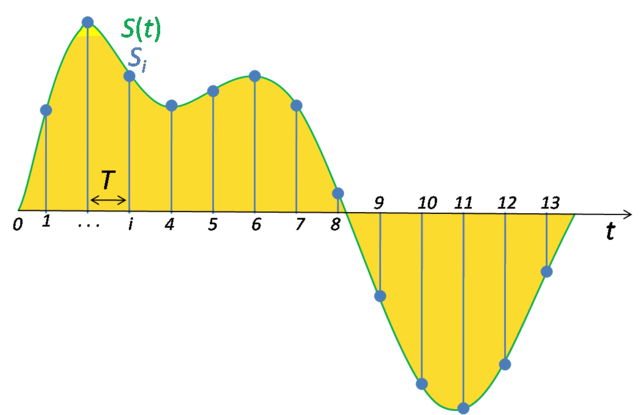
\includegraphics[width=0.6\textwidth]{Signal_Sampling}
%  \caption{Δειγματοληψία ενός αναλογικού σήματος}
%  \label{fig:sampling}
%\end{figure}
%Κατά τη δειγματοληψία ``χάνουμε'' αρκετή από την πληροφορία που περιέχει το αναλογικό σήμα, καθώς οι τιμές που βρίσκονται μεταξύ των διαστημάτων $T_s$ όπου λαμβάνουμε δείγματα δε λαμβάνονται υπόψη. Ακόμη, λόγω της πεπερασμένης ακρίβειας των ψηφιακών συστημάτων για αναπαράσταση αριθμών, η τιμή που έχει το σήμα στρογγυλοποιείται στην πλησιέστερη (είτε μεγαλύτερη είτε μικρότερη) τιμή που μπορεί να αναπαραστήσει το σύστημά μας.
%
%Όπως γίνεται αντιληπτό, σε πολλές των περιπτώσεων η δειγματοληψία μπορεί να έχει καταστροφικές συνέπειες για το αναλογικό σήμα. Ωστόσο, υπό προϋποθέσεις, μπορεί να είναι αντιστρεπτή διαδικασία -- μπορούμε δηλαδή από τα δείγματα που έχουμε λάβει να επιστρέψουμε στην αναλογική μορφή του σήματος. Οι προϋποθέσεις αυτές ορίζονται από το θεώρημα \emph{Shannon-Nyquist} (\ref{thrm:shannon-nyquist}), ως:
%\\
%\begin{theorem}[Shannon-Nyquist]
%	\label{thrm:shannon-nyquist}
%	Ένα σήμα με μέγιστη συχνότητα $f_{max}$ μπορεί να ανακτηθεί από τα δείγματά του, αν αυτά ληφθούν με συχνότητα $f_s>2f_{max}$, ή αλλιώς με περίοδο $T_s<\frac{1}{2f_{max}}$. \cite{proakis_sampling}
%\end{theorem}

\clearemptydoublepage

\chapter{Ρύθμιση του PID ελεγκτή}\label{ch:chap3}
%!TEX root = ../main.tex



\section{Εισαγωγή}

\lettrine[findent=2pt]{\fbox{\textbf{Η}}}{} ρύθμιση του PID ελεγκτή έχει να κάνει με την απόδοση τιμών στο συντελεστή κάθε όρου, έτσι ώστε καθένας από αυτούς να επηρεάσει θετικά την απόκριση του συστήματος, ενώ ταυτόχρονα να μετριαστούν όσο γίνεται περισσότερο τα αρνητικά του κάθε όρου. Ο τύπος της διεργασίας επηρεάζει το τι είναι επιθυμητό από τον έλεγχό της. Για παράδειγμα, κάποιες διεργασίες μπορεί να μην ανέχονται υπέρβαση (\emph{overshoot}) της απόκρισής τους και αυτό να θέτει και περιορισμούς στο χρόνο ανύψωσης (\emph{rise time}). Αντιθέτως, άλλες διεργασίες μπορεί να παρουσιάζουν ανοχή σε ένα ποσοστό υπέρβασης και έτσι να επιτρέπουν να αυξηθεί ο χρόνος ανύψωσης.

Παρόλο που η υλοποίηση του PID ελεγκτή είναι σχετικά ευθύς και απλή διαδικασία, η σωστή ρύθμισή του είναι πιο περίπλοκο ζήτημα. Αυτό συμβαίνει επειδή απαιτεί κατανόηση του τρόπου με τον οποίο κάθε όρους του PID επηρεάζει τη συνολική απόκριση. Ένας κακώς ρυθμισμένος PID ελεγκτής θα εμφανίσει αρκετά προβλήματα απόδοσης όπως: ταλαντώσεις, μη επαρκή απόσβεση, υπέρβαση, αργούς χρόνους ανόδου ή καθόδου και άλλα. Σε αυτό το κεφάλαιο θα γίνει μια περιγραφή κάποιων διαδεδομένων τεχνικών ρύθμισης που συναντάει κανείς στη βιβλιογραφία (υπάρχουν πολλές πιο εξελιγμένες μέθοδοι ρύθμισης αλλά υπόκεινται σε εμπορικές πατέντες) καθώς και των προβλημάτων που οφείλονται σε κακή ρύθμιση του PID ελεγκτή.

Η ανάλυση των τεχνικών ρύθμισης θα γίνει με αναφορά στα κέρδη $K_p$, $K_i$ και $K_d$, δηλαδή θα αφορά την παράλληλη μορφή του PID ελεγκτή της Εξίσωσης (\ref{eq:parallel_pid}) και όχι την τυποποιημένη μορφή της Εξίσωσης (\ref{eq:standard_pid}), παρόλο που η δεύτερη χρησιμοποιήθηκε στην εργασία αυτή. Αυτό συμβαίνει γιατί ο αναγνώστης είναι πιο εύκολο να καταλάβει πώς επηρεάζουν τα κέρδη την απόκριση του συστήματος χρησιμοποιώντας την πρώτη εξίσωση. Φυσικά, οι ίδιοι κανόνες ισχύουν και για τις παραμέτρους $T_i$ και $T_d$ της τυποποιημένης μορφής, έχοντας πάντα υπόψιν τις εξισώσεις που συνδέουν τις παραμέτρους των δύο αυτών σχέσεων.

\section{Τεχνικές ρύθμισης}

\subsection{Χειροκίνητη ρύθμιση}

Η πρώτη και πιο φυσική μέθοδος είναι η χειροκίνητη ρύθμιση του ελεγκτή από έναν χειριστή. Σε αυτή τη μέθοδο αρχικά τα κέρδη $K_i$ και $K_d$ ισούνται με το μηδέν. Στη συνέχεια, αυξάνουμε το αναλογικό κέρδος $K_p$ μέχρι το σύστημα να αρχίσει να ταλαντώνεται ελαφρώς και ο χρόνος ανύψωσης να είναι ικανοποιητικός. Έπειτα, αυξάνουμε το ολοκληρωτικό κέρδος $K_i$ έως ότου να εξαλειφθεί το σφάλμα μόνιμης κατάστασης, σε λογικό χρόνο για τη συγκεκριμένη διεργασία. Σε αυτό το σημείο πρέπει να έχουμε στο μυαλό μας ότι μεγαλύτερο ολοκληρωτικό κέρδος σημαίνει και μεγαλύτερη αστάθεια του συστήματος. Τέλος, αν χρειάζεται, αυξάνουμε το κέρδος παραγώγου $K_d$ για να βελτιώσουμε τη σταθερότητα του συστήματος καθώς και την απόκρισή του σε αλλαγή φορτίου ή σε κάποια διαταραχή. Εδώ πρέπει να έχουμε υπόψη μας ότι μεγάλο κέρδος παραγώγου θα προκαλέσει υπερβολική ανταπόκριση σε μεταβολές και υπέρβαση.

Ένας βρόχος PID που έχει ρυθμιστεί για να επιτύχει μια γρήγορη απόκριση συνήθως θα υπερβεί ελαφρώς την επιθυμητή τιμή ως συνέπεια της γρήγορης ``ρύθμισης" του. Εντούτοις, μερικά συστήματα δεν μπορούν να ανεχθούν οποιαδήποτε υπέρβαση, οπότε στην περίπτωση αυτή απαιτείται σύστημα κλειστού βρόχου, το οποίο θα πρέπει να έχει μικρότερο αναλογικό κέρδος $K_p$ από αυτό ενός συστήματος που μπορεί να ανεχτεί κάποιο ποσοστό υπέρβασης. Στον Πίνακα \ref{table:parameters} φαίνεται πώς ο κάθε όρος του ελεγκτή επηρεάζει την απόκριση του συστήματος υπό έλεγχο.

\begin{table}[H]
\begin{center}
\begin{tabular}{ |c|c|c|c|c|c| }
\hline
\thead{Παράμετρος} & \thead{Χρόνος \\ ανύψωσης} & \thead{Υπέρβαση} & \thead{Μόνιμο \\ σφάλμα} & \thead{Χρόνος \\ ηρεμίας} & \thead{Ευστάθεια}\\ \hline
\thead{$K_p$} & \thead{Μείωση} & \thead{Αύξηση} & \thead{Μείωση} & \thead{Μικρή \\ αλλαγή} & \thead{Χειροτέρευση} \\ \hline
\thead{$K_i$} & \thead{Μείωση} & \thead{Αύξηση} & \thead{Εξάλειψη} & \thead{Αύξηση} & \thead{Χειροτέρευση} \\ \hline
\thead{$K_d$} & \thead{Μικρή \\ αλλαγή} & \thead{Μείωση} & \thead{Καμία \\ αλλαγή} & \thead{Μείωση} & \thead{Βελτίωση} \\
\hline
\end{tabular}
\caption{Επίδραση στο σύστημα, της αύξησης κάθε παραμέτρου ανεξάρτητα από τις άλλες}
\label{table:parameters}
\end{center}
\end{table}

\subsection{Μέθοδος Ziegler–Nichols}

Ίσως η πιο γνωστή μέθοδος ρύθμισης ενός PID ελεγκτή είναι η \emph{Ziegler-Nichols}. Η μέθοδος αυτή έχει πάρει το όνομά της από τους \emph{John G. Ziegler} και \emph{Nathaniel B. Nichols} που την παρουσίασαν το $1942$ και χρησιμοποιείται ακόμα και σήμερα. Όπως και στην προηγούμενη μέθοδο, στην αρχή τα κέρδη $K_i$ και $K_d$ τίθενται ίσα με το μηδέν. Στη συνέχεια αυξάνουμε το κέρδος $K_p$ μέχρι το σύστημα αυξάνεται μέχρι την τιμή που θα οδηγήσει το σύστημα να εκτελεί ταλαντώσεις σταθερού πλάτους και σταθερής περιόδου. Η τιμή αυτή του κέρδους ονομάζεται απόλυτο κέρδος, $\boldsymbol{K_u}$, και η περίοδος των ταλαντώσεων ονομάζεται απόλυτη περίοδος, $\boldsymbol{T_u}$. Αυτές τις δύο παραμέτρους τις χρησιμοποιούμε για να ορίσουμε τα κέρδη όπως φαίνεται στον Πίνακα \ref{table:zn_method}. Στον πίνακα αυτόν έχουν υπολογιστεί οι παράμετροι $T_i$ και $T_d$ της τυποποιημένης μορφής του PID αλγορίθμου \cite{ziegler-nichols}. Αυτό έγινε επειδή αυτή η μορφή των παραμέτρων θα χρησιμοποιηθεί αργότερα για την αυτόματη ρύθμιση του ελεγκτή της εργασίας.


\begin{table}[H]
 \begin{center}
 \begin{tabular}{|c|c|c|c|}
 \hline
 Τύπος ελέγχου & $K_p$ & $T_i$ & $T_d$ \\ \hline
 P & $0.50K_u$ & -- & -- \\ \hline
 PI & $0.45K_u$ & $T_u/1.2$ & -- \\ \hline
 PD & $0.80K_u$ & -- & $T_u/8$ \\ \hline
 PID & $0.60K_u$ & $T_u/2$ & $T_u/8$ \\ \hline
 \end{tabular}
 \caption{Παράμετροι Ziegler-Nichols ανάλογα τον τύπο του ελεγκτή}
 \label{table:zn_method}
 \end{center}
\end{table}

Οι κανόνες ρύθμισης Ziegler-Nichols, συνήθως οδηγούν σε συστήματα με ιδιαίτερα υψηλή υπέρβαση και ``επιθετική" (``aggressive") απόκριση. Δεν παρέχουν δηλαδή μια έτοιμη λύση ρύθμισης αλλά τις περισσότερες φορές προσφέρουν ένα αρκετά ικανοποιητικό σημείο εκκίνησης από το οποίο ο χειριστής μπορεί να ξεκινήσει να τροποποιεί τα κέρδη έτσι ώστε να έχει την επιθυμητή απόκριση.

\subsection{Μέθοδος Tyreus-Luyben}

Μια μέθοδος πολύ παρόμοια με τη μέθοδο Ziegler-Nichols που περιγράφηκε πριν είναι η μέθοδος Tyreus-Luyben. Και αυτή βασίζεται στην απόλυτη συχνότητα (\emph{$T_u$}) και στο απόλυτο κέρδος (\emph{$K_u$}) του συστήματος. Το μόνο που αλλάζει σε σχέση με την προηγούμενη μέθοδο είναι οι τιμές των κερδών ανάλογα με τον τύπο ελέγχου. Οι τιμές αυτές φαίνονται στον Πίνακα \ref{table:tl_method}.

\begin{table}[H]
 \begin{center}
 \begin{tabular}{|c|c|c|c|}
 \hline
 Τύπος ελέγχου & $K_p$ & $T_i$ & $T_d$ \\ \hline
% P & $0.50K_u$ & - & - \\ \hline
 PI & $K_u/3.2$ & $2.2T_u$ & -- \\ \hline
% PD & $0.80K_u$ & - & $T_u/8$ \\ \hline
 PID & $K_u/2.2$ & $2.2T_u$ & $T_u/6.3$ \\ \hline
 \end{tabular}
 \caption{Παράμετροι Tyreus-Luyben ανάλογα τον τύπο του ελεγκτή}
 \label{table:tl_method}
 \end{center}
\end{table}

\subsection{Μέθοδος Cohen-Coon}

Αυτή η μέθοδος αναπτύχθηκε το $1953$ και βασίζεται σε ένα μοντέλο συστήματος πρώτης τάξης με μία χρονοκαθυστέρηση. Παρόμοια με τη μέθοδο Ziegler-Nichols, η μέθοδος αυτή προτείνει ένα σύνολο παραμέτρων συντονισμού για να δώσει μια απόκριση κλειστού βρόχου με λόγο απόσβεσης $1/4$. Σε αντίθεση όμως με τις δύο προηγούμενες μεθόδους που χρησιμοποιούν στοιχεία της απόκρισης συχνότητας του συστήματος για να βγάλουν υπολογίσουν τα κέρδη του ελεγκτή, αυτή η χρησιμοποιεί στοιχεία από την βηματική απόκριση (\emph{Step response}) του συστήματος.

\subsection{Άλλες μέθοδοι και περαιτέρω πληροφορίες}

Στην ενότητα αυτή περιγράφηκαν οι πιο γνωστές και διαδεδομένες τεχνικές ρύθμισης ενός PID ελεγκτή. Βέβαια τα πολλά χρόνια εφαρμογής των PID ελεγκτών στη βιομηχανία, καθώς και η ανάγκη για όλο και πιο λεπτομερή και στιβαρό έλεγχο έχουν οδηγήσει στην ανάπτυξη πολλών ακόμα μεθόδων και τεχνικών. Βέβαια πολλές από αυτές προστατεύονται από νόμους περί πνευματικής ιδιοκτησίας. Εδώ αναλύθηκαν μόνο οι μέθοδοι που χρησιμοποιήθηκαν στο πρακτικό κομμάτι της εργασίας. Κάποιος που ενδιαφέρεται για μια αναλυτική προσέγγιση σε πολλές μεθόδους ρύθμισης καθώς και να μάθει για τα πλεονεκτήματα και τους περιορισμούς της κάθε μίας μπορεί να ανατρέξει στις πηγές \cite{astrom}, \cite{yun}, \cite{kristian}.

\section{Περιορισμοί και προβλήματα κακής ρύθμισης}

\lettrine[findent=2pt]{\fbox{\textbf{Π}}}{αρόλο} που οι ελεγκτές PID είναι εφαρμόσιμοι σε πολλά προβλήματα ελέγχου και συχνά παρέχουν ικανοποιητικό έλεγχο χωρίς βελτιώσεις ακόμα και όταν έχουν ρυθμιστεί ``στο περίπου", μπορούν να έχουν χαμηλή απόδοση σε ορισμένες εφαρμογές και σχεδόν ποτέ δεν παρέχουν βέλτιστο έλεγχο. Η βασική δυσκολία με τον έλεγχο PID είναι ότι είναι ένα σύστημα ελέγχου ανατροφοδότησης, με σταθερές παραμέτρους και χωρίς άμεση γνώση της διαδικασίας και έτσι η συνολική απόδοση είναι αντιδραστική και συμβιβαστική.

Οι ελεγκτές PID, όταν χρησιμοποιούνται μόνοι τους, μπορούν να έχουν χαμηλή απόδοση όταν τα κέρδη τους πρέπει να μειωθούν, έτσι ώστε το σύστημα ελέγχου να μην παρουσιάζει υπέρβαση, να μην ταλαντώνεται ή να μην κυνηγάει την τιμή ρύθμισης του ελέγχου. Παρουσιάζουν επίσης προβλήματα όταν εμφανίζονται μη γραμμικότητες, μπορεί να ανταλλάσουν την πιο ομαλή απόκριση έναντι του χρόνου απόκρισης, να μην αντιδρούν στην αλλαγή της συμπεριφοράς της διαδικασίας (ας πούμε, η διαδικασία αλλάζει μετά από το ζέσταμα) και να έχουν καθυστέρηση στην αντιμετώπιση μεγάλων διαταραχών.

\subsection{Γραμμικότητα}

Ο PID ελεγκτής είναι ένα γραμμικό και ιδιαίτερα συμμετρικό σύστημα. Συνεπώς, η απόκρισή του όταν εφαρμόζεται σε ένα μη γραμμικό σύστημα είναι μεταβλητή. Για παράδειγμα, στον έλεγχο της θερμοκρασίας, μια κοινή περίπτωση χρήσης είναι η ενεργή θέρμανση (μέσω θερμαντικού στοιχείου), αλλά η παθητική ψύξη (θέρμανση χωρίς ψύξη), οπότε η υπέρβαση που μπορεί να προκαλεί ο ελεγκτής διορθώνεται αργά - δεν μπορεί να εξαναγκαστεί προς τα κάτω. Σε αυτή την περίπτωση ο PID θα πρέπει να ρυθμιστεί ώστε να παρέχει υπεραποσβενούμενη απόκριση, για να αποτρέψει ή να μειώσει την υπέρβαση, αν και αυτό μειώνει την απόδοση του συστήματος (αυξάνει το χρόνο ηρεμίας).

\subsection{Θόρυβος στον παράγωγο όρο}

Ένα πρόβλημα με τον παράγωγο όρο είναι ότι ενισχύει τη μέτρηση υψηλής συχνότητας ή το θόρυβο της διαδικασίας, με αποτέλεσμα να προκαλούνται μεγάλες αλλαγές στην έξοδο. Συχνά είναι χρήσιμο να φιλτράρονται οι μετρήσεις με φίλτρο χαμηλής διέλευσης (\emph{low-pass filter}) για να αφαιρείται ο θόρυβος υψηλής συχνότητας. Καθώς το φιλτράρισμα χαμηλής διέλευσης και ο παράγωγος έλεγχος μπορούν να ακυρώνουν ο ένας στον άλλο, η ποσότητα φιλτραρίσματος είναι περιορισμένη. Μπορεί επίσης να χρησιμοποιηθεί ένα μη γραμμικό διάμεσο φίλτρο, το οποίο βελτιώνει την αποδοτικότητα φιλτραρίσματος και την πρακτική απόδοση \cite{chong}. Σε ορισμένες περιπτώσεις, ο παράγωγος όρος μπορεί να απενεργοποιηθεί με λίγες διαφοροποιήσεις στη συνολική απόδοση.

\subsection{Ταλαντώσεις}

Η ταλάντωση είναι ένα από τα πιο περίπλοκα ζητήματα επίδοσης στους PID ελεγκτές και μπορεί να είναι αποτέλεσμα πολλών παραγόντων. Η πιο συνηθισμένη αιτία είναι το πολύ μεγάλο αναλογικό κέρδος (Σχήμα \ref{fig:proportional_oscillation}). Μια δεύτερη αιτία είναι ένας ελεγκτής που βασίζεται κυρίως στον ολοκληρωτικό του όρο (Σχήμα \ref{fig:integral_oscillations}) επειδή το σφάλμα που έχει συσσωρευτεί ενώ η μετρούμενη μεταβλητή είναι κάτω από το καθορισμένο σημείο χρειάζεται χρόνο για να διορθωθεί ενώ η μετρούμενη μεταβλητή είναι πάνω από το καθορισμένο σημείο. Ο ολοκληρωτικός όρος στη συνέχεια αρχίζει να συσσωρεύει σφάλμα στην αντίθετη κατεύθυνση, το οποίο δεν θα διορθωθεί μέχρις ότου η μετρούμενη μεταβλητή να διασχίσει ξανά το καθορισμένο σημείο. Σε αυτή την περίπτωση ο αναλογικός όρος ενεργεί ως αποσβεστήρας. Τρίτον, κάτι που εύκολα παραβλέπεται πολλές φορές, είναι ότι το το φυσικό σύστημα που ελέγχεται θα μπορούσε να έχει από μόνο του ταλαντευόμενο χαρακτήρα και συνεπώς η ύπαρξη ταλαντώσεων στο σύστημα ίσως είναι αποδεκτή. Αυτό δεν σημαίνει απαραίτητα κακή ρύθμιση του PID ελεγκτή.

\begin{figure}[h]
  \centering
  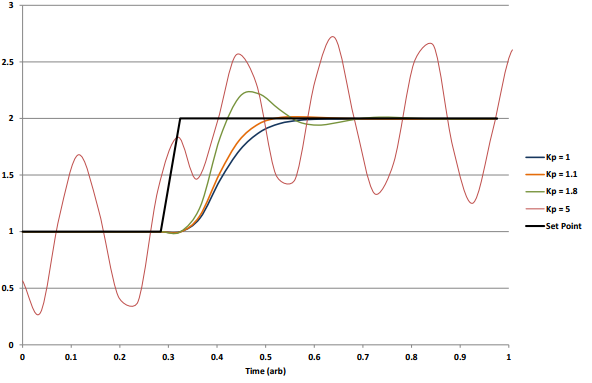
\includegraphics[width=\textwidth]{proportional_oscillation}
  \caption{Απόκριση της μετρούμενης μεταβλητής στην αύξηση του αναλογικού κέρδους}
  \label{fig:proportional_oscillation}
\end{figure}

\begin{figure}[h]
  \centering
  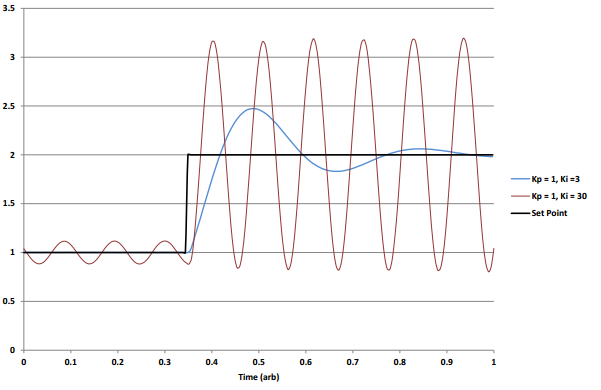
\includegraphics[width=\textwidth]{integral_oscillations}
  \caption{Ταλαντώσεις λόγω υψηλού ολοκληρωτικού κέρδους}
  \label{fig:integral_oscillations}
\end{figure}

Η συχνότητα του ελεγκτή είναι ο ρυθμός με τον οποίο ο βρόχος ελέγχου λειτουργεί και η έξοδος τροφοδοσίας ενημερώνεται μία φορά ανά κύκλο. Αυτή η συμπεριφορά απλής ενημέρωσης μπορεί να είναι προβληματική αν το αναλογικό κέρδος είναι υπερβολικά υψηλό. Ένα μικρό σφάλμα παράγει μια μεγάλη έξοδο, η οποία προκαλεί μεγάλη μεταβολή στη μετρούμενη μεταβλητή, ακόμη και σε έναν κύκλο. Εάν η αλλαγή αυτή μεταβάλλει τη μετρούμενη μεταβλητή πέρα από το καθορισμένο σημείο, τότε η έξοδος αντιστρέφει την πολικότητα για τον επόμενο κύκλο. Αν η μετρούμενη μεταβλητή συνεχίζει να πηδάει από το κύκλο σε κύκλο, τότε ο ελεγκτής ταλαντώνεται. Αν το κέρδος είναι αρκετά υψηλό και προκαλεί την μεταπήδηση της μετρούμενης μεταβλητής με αυξανόμενο μέγεθος σφάλματος, τότε ο ελεγκτής θεωρείται ασταθής. Η πιο γρήγορη λύση είναι η μείωση του αναλογικού κέρδος. Ωστόσο, η αύξηση της συχνότητας του ελεγκτή, αν αυτό είναι δυνατόν, θα βοηθήσει επίσης.

Αυτός είναι εγγενής περιορισμός ενός ψηφιακού ελεγκτή. Θα υπάρχει πάντα ταλάντωση σε κάποιο βαθμό. Εκτός από το ζήτημα συχνότητας βρόχου που έχει ήδη περιγραφεί, η έξοδος της τροφοδοσίας μπορεί να μειωθεί μόνο σε κάποια πεπερασμένη τιμή και τίποτα μικρότερο. Το πρόβλημα τότε γίνεται ζήτημα πόσο μπορεί να μειωθεί η ταλάντωση. Ένας απόλυτα συνεχής ελεγκτής δεν έχει αυτό το πρόβλημα επειδή η έξοδος συνεχώς ενημερώνεται μαζί με το μεταβαλλόμενο σφάλμα. Ωστόσο, η ταλάντωση από τους περιορισμούς συχνότητας εξακολουθεί να συμβαίνει στον συνεχή έλεγχο PID. Αυτοί οι ελεγκτές είναι αναλογικά κυκλώματα και εξακολουθούν να έχουν μια αποτελεσματική συχνότητα λειτουργίας που προκύπτει από αντιδραστικά στοιχεία που προκαλούν χρονική υστέρηση μεταξύ της εξόδου και της εισόδου.

Η ταλάντωση λόγω ενός υψηλού ολοκληρωτικού κέρδους μπορεί να μειωθεί είτε μειώνοντας το ολοκληρωτικό κέρδος (προφανής λύση) είτε αυξάνοντας το αναλογικό κέρδος (όχι άμεσα προφανές). Η αναλογική δράση θα επιβραδύνει τις ταλαντώσεις που προκαλούνται από την ολοκληρωτική δράση. Αυτό το παράδειγμα παρουσιάζει τη δυσκολία συντονισμού του PID ελεγκτή. Ο χρήστης πρέπει να αποφασίσει ποια χαρακτηριστικά των αποκρίσεων του ελεγκτή είναι απαραίτητα, επιθυμητά και ποια είναι μη αποδεκτά. Κάθε όρος έχει υπέρ και κατά και πρέπει να καθοριστεί η προτεραιότητα των χαρακτηριστικών του ελεγκτή πριν από την προσπάθεια ρύθμισης του συστήματος.

\subsection{Χρόνος ανόδου και Υπέρβαση}

Ο χρόνος ανόδου της μετρούμενης μεταβλητής είναι ο χρόνος που απαιτείται για την μετρούμενη μεταβλητή να φτάσει στο καθορισμένο σημείο μετά από μια αλλαγή. Ένας γρήγορος χρόνος ανόδου είναι επιθυμητός για προφανείς λόγους, αλλά ένας πολύ μικρός χρόνος ανόδου θα προκαλέσει υπέρβαση της μετρούμενης μεταβλητής από το καθορισμένο σημείο. Η υπέρβαση μπορεί στη συνέχεια να μετατραπεί σε αποσβενούμενες ταλαντώσεις για όσο χρονικό διάστημα η μετρούμενη μεταβλητή προσπαθεί να ισορροπήσει στο καθορισμένο σημείο. Για κάποιες εφαρμογές, μια μικρή υπέρβαση είναι αποδεκτή παραχώρηση έτσι ώστε να επιτευχθεί ένας μικρός χρόνος ανόδου. Για άλλες διεργασίες, καμία υπέρβαση δεν είναι ανεκτή και η προσεκτική επιλογή των κερδών του PID ελεγκτή πρέπει να έχει ως αποτέλεσμα τον ταχύτερο χρόνο ανόδου χωρίς υπέρβαση. 

Ο χρόνος ανόδου επηρεάζεται κυρίως από το αναλογικό και το παράγωγο κέρδος. Η παράγωγος ενέργεια αντιδρά έντονα σε μία απότομη αλλαγή αλλά επιβραδύνει την προσέγγιση στο καθορισμένο σημείο. Η ολοκληρωτική συνιστώσα δεν επηρεάζει αισθητά τον χρόνο ανόδου λόγω της φύσης της που αφορά τη συσσώρευση σφάλματος, αλλά μπορεί να προκαλέσει υπέρβαση. Επιπλέον, όπως περιγράφηκε προηγουμένως, θα υπάρξει ένα μεγάλο ενιαίο κέρδος προκαλούν ταλαντώσεις. 

Ο χρόνος άνοδος τυπικά ορίζεται ως ο χρόνος για την αύξηση της μεταβλητής ενδιαφέροντος από $10\%$ της τελικής τιμής στο $90\%$ της τελικής τιμής. Αυτός είναι ο ορισμός που χρησιμοποιείται εδώ.


%\section{Μοντελοποίηση προβλήματος}
%
%\lettrine[findent=2pt]{\fbox{\textbf{Π}}}{ριν} δούμε στην πράξη πώς λειτουργούν οι τεχνικές super resolution θα πρέπει να περιγράψουμε το πρόβλημα με το οποίο θα δουλέψουμε με μαθηματικούς όρους. Η μοντελοποίηση αυτή θα μας επιτρέψει να χρησιμοποιήσουμε μαθηματικά εργαλεία και τεχνικές και να ορίσουμε σε μια αυστηρή ``γλώσσα'' (αυτή των μαθηματικών) τις λειτουργίες που επιτελούνται από κάθε μέθοδο, ούτως ώστε να πετύχουμε το τελικό αποτέλεσμα.
%
%Ξεκινώντας, θα πρέπει να περιγράψουμε τον τρόπο με τον οποίο λαμβάνουμε εικόνες χαμηλής ανάλυσης από μια φυσική σκηνή μέσω μιας κάμερας. Η κάμερα σαν όργανο καταγραφής εισάγει κάποιες ατέλειες, όπως είδαμε στο προηγούμενο κεφάλαιο. Τέτοιες ατέλειες μπορεί να είναι σφάλματα καταγραφής από τον αισθητήρα της κάμερας, θόλωμα λόγω αστοχιών των οπτικών στοιχείων κλπ. Επιπλέον, αν λάβουμε διαδοχικές εικόνες μιας φυσικής σκηνής, οι εικόνες αυτές περιμένουμε να έχουν κάποιες μετατοπίσεις ως προς αυτό που απεικονίζουν. Οι μετατοπίσεις αυτές μπορεί να οφείλονται είτε στον άνθρώπινο παράγοντα (που χειρίζεται την κάμερα) είτε στο αντικείμενο της φυσικής σκηνής που μπορεί να μην είναι σταθερό. Στην εικόνα που λαμβάνεται τελικά, λαμβάνονται δείγματα σε χαμηλή χωρική συχνότητα και λόγω ατελειών του οργάνου μπορεί να έχουμε και παρουσία θορύβου. Για μια εικόνα υψηλής ανάλυσης $\bm{X}$ (την οποία θα προσπαθήσουμε να ανακατασκευάσουμε), μπορούμε να αναπτύξουμε το παραπάνω μοντέλο ως εξής:
%\begin{equation} \label{eq:hrmodel}
%\bm{Y}_i=\bm{S}_i\bm{T}_i\bm{H}_i\bm{X}+\bm{n}_i
%\end{equation}
%όπου ορίζουμε για την i-οστή εικόνα χαμηλής ανάλυσης $\bm{Y}_i$ τους τελεστές που ενεργούν στην $\bm{X}$ : 
%\begin{itemize}
%	\item $\bm{S}_{i}$ για υποδειγματοληψία, 
%	\item $\bm{T}_{i}$ για μετατόπιση, 
%	\item $\bm{H}_{i}$ για θόλωμα (blurring), 
%	\item $\bm{n_{i}}$ για προσθετικό θόρυβο.
%\end{itemize}
%Οι υποθέσεις που κάνουμε για το παραπάνω πρόβλημα είναι ότι το blurring είναι ίδιο σε όλο το χώρο και είναι γνωστό στον αλγόριθμο super resolution, ο θόρυβος είναι λευκός Gaussian με την ίδια διασπορά σε όλες τις εικόνες χαμηλής ανάλυσης και ότι ο γεωμετρικός μετασχηματισμός αφορά μόνο την καθολική μετατόπιση. 
%
% Στην περίπτωση που θεωρήσουμε αμελητέο θόρυβο και θόλωμα, τα παραπάνω βήματα αρκούν για να υπολογίσουμε την εικόνα υψηλής ανάλυσης $\bm{X}$, την οποία λαμβάνουμε σαν αποτέλεσμα του αλγορίθμου.
%
%\begin{algorithm}
%
% \KwData{$\bm{dx}$, $\bm{dy}$, $\bm{Y}_i$, $N$, $W$, $\bm{H}$, $S$}
% \KwOut{High resolution reconstructed $\bm{X}$}
% $\bm{X} \gets 0$\; 
% \For{$n \gets 1$ \textbf{to} $N$}{
% 	$\bm{\tilde{Y}} \gets \bm{Y}_i$\;
%    $\bm{i} \gets 1:W/S$\;
%    $\bm{j} \gets 1:H/S$\;
%    $\bm{px}=\bm{i}*S+\bm{dx}_n$\;
%    $\bm{py}=\bm{j}*S+\bm{dy}_n$\;
%    $\bm{X}_{px,py}=\bm{\tilde{Y}}_{i,j}$\;
%    }
%    %\vspace{-1.5em}
% \caption{Ανακατασκευή shift-add fusion}\label{algo:sr_fusion}
%\end{algorithm}
%
%Συγκρίνοντας τη μέθοδο αυτή με την ανακατασκευή μέσω του μετασχηματισμού Fourier, παρατηρούμε την απλότητα και την αποδοτικότητά της καθώς βρίσκει την εικόνα υψηλής ανάλυσης μόνο με μετακινήσεις pixel. 
\clearemptydoublepage

\chapter{Ο Αυτο-Ρυθμιζόμενος PID Ελεγκτής}\label{ch:chap4}
%!TEX root = ../main.tex



\section{Εισαγωγή}


\clearemptydoublepage

%!TEX root = ./main.tex

\begin{thebibliography}{99}

\bibitem{labview1} \url{https://en.wikipedia.org/wiki/LabVIEW}
\bibitem{labview2} \url{http://www.ni.com/en-us/shop/labview.html}
\bibitem{labview3} Jeffrey Travis, Jim Kring, “LabVIEW for Everyone: Graphical Programming Made Easy and Fun (3rd ed.)”, Prentice Hall Professional, July 27, 2006, ISBN-13: 978-0-13-185672-1.
\bibitem{dataflow_programming} Johnston, W.M., Hanna, J.R.P. and Millar, R.J. ``Advances in dataflow programming languages". ACM Computing Surveys 36 (1): 1–34. 2004. DOI: 10.1145/1013208.1013209




%\bibitem{keren} D. Keren, S. Peleg, and R. Brada, “Image sequence enhancement using subpixel
%displacements,” in IEEE Computer Society Conference on Computer Vision and
%Pattern Recognition, June 1988, pp. 742–746.
%\bibitem{hardie} R. Hardie, K. Barnard, and E. Armstrong, “Joint MAP registration and high resolution image estimation using a sequence of undersampled images,” IEEE Transactions on Image Processing, vol. 6, no. 12, pp. 1621–1633, December 1997.
%\bibitem{patti} A. Patti, M. Sezan, and A. Tekalp, “High-resolution image reconstruction from
%a low-resolution image sequence in the presence of time-varying motion blur,” in
%Proceedings of the IEEE International Conference on Image Processing, Austin,
%TX, vol. 1, 1994, pp. 343–347.
%\bibitem{hardie2} R. C. Hardie, K. J. Barnard, J. G. Bognar, E. E. Armstrong, and E. A. Watson, “High resolution image reconstruction from a sequence of rotated and translated
%frames and its application to an infrared imaging system,” Optical Engineering,
%vol. 37, no. 1, pp. 247–260, January 1998.
%\bibitem{alam} M. S. Alam, J. G. Bognar, R. C. Hardie, and B. J. Yasuda, “Infrared image registration and high-resolution reconstruction using multiple translationally shifted aliased video frames,” IEEE Transactions on Instrumentation and Measurement, vol. 49,
%no. 5, pp. 923–915, October 2000.
%\bibitem{tsai} R. Y. Tsai and T. S. Huang, “Multiframe image restoration and registration,” in Advances in Computer Vision and Image Processing: Image Reconstruction from Incomplete Observations, T. S. Huang, Ed., vol. 1. London: JAI Press, 1984, pp. 317–339.
%\bibitem{kim} N. K. Bose, H. C. Kim, and H. M. Valenzuela, “Recursive total least squares algorithm for image reconstruction from noisy undersampled frames,” Multidimensional Systems and Signal Processing, vol. 4, no. 3, pp. 253–268, July 1993.
%\bibitem{yang} J. Yang, J. Wright, T. Huang, and Yi Ma. Image super-resolution via sparse representation. IEEE Transactions on Image Processing (TIP), vol. 19, issue 11, 2010.
%\bibitem{ransac} Martin A. Fischler and Robert C. Bolles (June 1981). “Random Sample Consensus: A Paradigm for Model Fitting with Applications to Image Analysis and Automated Cartography”. Comm. of the ACM 24 (6): 381–395
%\bibitem{wired_ff_algo} Jordan Ellenberg, ”Fill in the Blanks: Using Math to Turn Lo-Res Datasets Into Hi-Res Samples”, 22 February 2010, Wired Magazine \url{http://www.wired.com/2010/02/ff_algorithm/}
%\bibitem{incoherence} D.L. Donoho and X. Huo, “Uncertainty principles and ideal atomic decomposition,” IEEE Trans. Inform. Theory, vol. 47, no. 7, pp. 2845–2862, Nov. 2001.
%\bibitem{candes} E. Candes, “Compressive sensing,” in Proceedings of the International Congress of Mathematicians, vol. 3, pp. 1433–1452, 2006.
%\bibitem{donoho} D. L. Donoho, “Compressed sensing,” IEEE Transactions on Information Theory, vol. 52, no. 4, pp. 1289–1306, 2006.
%\bibitem{proakis_sampling} John G. Proakis, Dimitris G. Manolakis , “Digital Signal Processing - Principles, Algorithms, Implementations” 4th edition (Pearson International Edition), Pearson Education, Chapter 1.4.2: The Sampling Theorem 
%\bibitem{gonzalez_2d_fft} Rafael C. Gonzalez, Richard E. Woods , “Digital Image Processing” 3rd edition (Pearson International Edition), Pearson Education, Chapter 1.4.2: The 2D Discrete Fourier Transform and its Inverse
%\bibitem{shift_add_fusion} S. Farsiu, M. Elad, P. Milanfar, “Fast and Robust Multiframe Super Resolution” IEEE Transactions on Image Processing, vol. 13, no. 10, October 2004
%\bibitem{imregintro} ”Image Registration", in Wikipedia: The Free Encyclopedia; (Wikimedia Foundation Inc., updated 2 December 2014, 15:50 UTC) \url{http://en.wikipedia.org/wiki/Image_registration}
%\bibitem{cs_intro} M. Davenport, M. Duarte, Y. Eldar, G. Kutyniok, ”Introduction to Compressed Sensing”, Stanford University - Department of Statistics
%\bibitem{convexmin} F. Bach, R. Jenatton, J. Mairal, G. Obozinski, ”Convex Optimization with Sparsity-Inducing Norms”, Institut National de Recherche en Informatique et en Automatique (INRIA)
%\bibitem{red_dict} H. Rauhut, K. Schnass, and P. Vandergheynst, “Compressed sensing and redundant dictionaries,” IEEE Transactions on Information Theory, vol. 54, no. 5, May 2008.
%\bibitem{denoising_dict} M. Elad and M. Aharon, “Image denoising via sparse and redundant representations over learned dictionaries,” IEEE Transactions on Image Processing, vol. 15, pp. 3736–3745, 2006.
%\bibitem{im_vid_rest} J. Mairal, G. Sapiro, and M. Elad, “Learning multiscale sparse representations for image and video restoration,” Multiscale Modeling and Simulation, vol. 7, pp. 214–241, 2008.
%\bibitem{ksvd_dict} M. Aharon, M. Elad, and A. Bruckstein, “K-SVD: An algorithm for designing overcomplete dictionaries for sparse representation,” IEEE Transactions on Signal Processing, vol. 54, no. 11, pp. 4311–4322, Nov. 2006.
%\bibitem{sparse_coding_dict} H. Lee, A. Battle, R. Raina, and A. Y. Ng, “Efficient sparse coding algorithms,” in Advances in Neural Information Processing Systems (NIPS), pp. 801–808, 2007.
%\bibitem{human_sparse} B. Olshausen and D. Field, “Sparse coding with an overcomplete basis set: A strategy employed by V1?,” Vision Research, vol. 37, no. 23, pp. 3311–3325, 1997.
%\bibitem{nphard} ”NP-hard", in Wikipedia: The Free Encyclopedia; (Wikimedia Foundation Inc., updated 9 April 2015, 15:30 UTC) \url{http://en.wikipedia.org/wiki/NP-hard}
%\bibitem{nphard1} D. L. Donoho, “For most large underdetermined systems of linear equations, the minimal $l_1$-norm solution is also the sparsest solution,” Communications on Pure and Applied Mathematics, vol. 59, no. 6, pp. 797–829, 2006.
%\bibitem{nphard2} “For most large underdetermined systems of linear equations, the minimal $l_1$-norm near-solution approximates the sparsest near-solution,” Communications on Pure and Applied Mathematics, vol. 59, no. 7, pp. 907–934, 2006.
%\bibitem{lasso} R. Tibshirani, “Regression shrinkage and selection via the lasso,” Jour- nal of Royal Statistical Society, Series B, vol. 58, no. 1, 1996.
%\bibitem{dict_training} Jianchao Yang, Zhaowen Wang, Zhe Lin, and Thomas Huang. Coupled dictionary training for image super-resolution. IEEE Transactions on Image Processing (TIP), vol. 21, issue 8, pages 3467-3478, 2012.
%\bibitem{srexample} W. T. Freeman, T. R. Jones, and E. C. Pasztor, “Example-based superresolution,” IEEE Computer Graphics and Applications, vol. 22, pp. 56–65, 2002.
%\bibitem{lowlevel} W. T. Freeman, E. C. Pasztor, and O. T. Carmichael, “Learning low-level vision,” International Journal of Computer Vision, vol. 40, no. 1, pp. 25–47, 2000.
%\bibitem{sr_neigh} H. Chang, D.-Y. Yeung, and Y. Xiong, “Super-resolution through neighbor embedding,” in IEEE Conference on Computer Vision and Pattern Classifi- cation (CVPR), vol. 1, pp. 275–282, 2004.
%\bibitem{imhal} J. Sun, N. N. Zheng, H. Tao, and H. Shum, “Image hallucination with primal sketch priors,” in IEEE Conference on Computer Vision and Pattern Recognition (CVPR), vol. 2, 2003, pp. 729–736.
%\bibitem{imfill} imfill, Image Processing Toolbox Documentation, MathWorks \\ \url{http://www.mathworks.com/help/images/ref/imfill.html}
%\bibitem{imresize} imresize, Image Processing Toolbox Documentation, MathWorks \\ \url{http://www.mathworks.com/help/images/ref/imresize.html}
%\bibitem{k-term} A. Cohen, W. Dahmen, R. DeVorce, "Compressed sensing and best k-term approximation", in the Journal of the American Mathematical Society, vol. 22, pp. 211-231 , 2009.




\end{thebibliography}

\clearemptydoublepage

\pagestyle{empty}

\vspace*{\fill}
%\hline
\begin{flushleft}
	Πανεπιστήμιο Πατρών, Πολυτεχνική Σχολή \\
	Τμήμα Ηλεκτρολόγων Μηχανικών και Τεχνολογίας Υπολογιστών \\
	{\nomme} \\
	© \monthyear \ -- Με την επιφύλαξη παντός δικαιώματος.\\
\end{flushleft}
%\hline


\end{document}
